\section{Methodology}

This methodology section details the overall analytical framework and specific techniques to be employed in this research.

The proposed methodology consists of the following key steps:

\begin{enumerate}
\item Dimension reduction on stressors that produce pollution scores and arranges samples in a low-dimensional pollutant space to reveal main synthetic stressor gradients.

\item Find and prepare least polluted sites, construct an estimator that estimates the counterfactual surface (minimal pollution level) of taxa community composition in environmental space.

\item Ordinate the taxa variables, construct comprehensive measurement for the taxa community.

\item Spatial heterogeneity test and geo-information incorporated for latent environmental variables.

\item Piecewise quantile regression models on ZCI and pollution scores, revealing relations at different quantile levels and detecting thresholds.

\item Step out of the framework, change global factors, like sample size and partitioning samples by biased environmental distribution. Study how the series of estimates would change accordingly.
\end{enumerate}

Various symbols are used throughout this section, including function names, vectors, and matrices. The following table summarizes these symbols:

\begin{table}[!h]
\centering
\caption{Summary of major mathematical symbols and their meanings, organized by subsection.}
\begin{tabular}{lll}
\toprule
\textbf{Subsection} & \textbf{Symbol} & \textbf{Meaning} \\
\midrule
\multirow{7}{*}{\parbox{3cm}{\centering Data Description and Sediment Contamination Assessment}} 
& $m$ & Number of sampled sites \\
& $X \in \mathbb{R}^{m \times 30}$ & Elemental concentration matrix (30 chemical elements) \\
& $E \in \mathbb{R}^{m \times 5}$ & Environmental variable matrix (5 variables) \\
& $T \in \mathbb{R}^{m \times 16}$ & Taxa abundance matrix (16 taxa) \\
& $s \in \mathbb{R}^m$ & Composite stressor score (from PCA) \\
& $p\%$ & Percentage of least stressed sites chosen as reference \\
& $I_{\mathrm{ref}} \in \mathbb{R}^m$ & Indicator: 1 = reference site, 0 = disturbed site \\
\midrule

\multirow{5}{*}{\parbox{3cm}{\centering Reference site clustering and Discriminant Function}} 
& $\mathcal{C}_K$ & Cluster label (taxa composition group) from reference sites \\
& $\hat{\mathcal{C}}_K$ & Predicted cluster label for disturbed sites \\
& $\mathcal{F}_{\mathrm{dis}}$ & Discriminant function mapping $E_{\mathrm{ref}}$ to $\mathcal{C}_K$ \\
& $\delta T_{i,j}$ & Taxa community structure relative to the scale of reference site \\
& $\delta X_{k,j}$ & Stress level relative to group-$k$ reference median \\
\midrule

\multirow{12}{*}{\parbox{3cm}{\centering
    Multivariate Gaussian modeling for constructing Zoobenthic Community Index (ZCI)
 }} 
& $\phi_{\mathrm{Hel}}$ & Hellinger transformation \\
& $\mathcal{R}_k$, $\mathcal{D}_k$ & Sets of reference and disturbed sites in group $k$ \\
& $\boldsymbol{\mu}_k$ & Mean taxa composition vector for group $k$ reference sites \\
& $\boldsymbol{\Sigma}_k$ & Covariance matrix of taxa composition in group $k$ \\
& $\lambda$ & Ridge regularization term \\
& $I_{16}$ & $16\times16$ identity matrix \\
& $\tilde{T}_{k,j}$ & Whitened deviation vector for site $j$ in group $k$ \\
& $\mathrm{ZCI}_{k,j}$ & Scalar Mahalanobis distance from reference centroid \\
& $\mathrm{ZCI}^{(\mathrm{diag})}_{k,j}$ & Diagonal approximation ignoring correlations \\
& $\mathrm{ZCI}^{(1)}_{k,j}, \mathrm{ZCI}^{(2)}_{k,j}$ & First two components of multi-dimensional ZCI \\
& $\mathrm{ZCI}^\star_{k,j}$ & 0--100 scaled ZCI score \\
& $V_k$ & PCA loading matrix from whitened reference deviations \\
\midrule

\multirow{4}{*}{\parbox{3cm}{\centering
    Spatial basis expansion for spatial predictors
}} 
& $x_i, y_i$ & Spatial coordinates of site $i$ \\
& $D \in \mathbb{R}^{m \times m}$ & Euclidean distance matrix(symmetrical) between sites \\
& $A \in \mathbb{R}^{m \times m}$ & Double-centered distance matrix from truncated distance matrix \\
& $S_{\text{sel}} \in \mathbb{R}^{m \times d}$ & Selected eigenvectors for explaining spatial variation (\(d < m\)) \\
\midrule

\multirow{7}{*}{\parbox{3cm}{\centering Quantile regression modeling}} 
& $\mathcal{F}_{k}$ & Regression function linking ZCI and spatial features to stress level \\
& $\delta X\mid Z, S_{\text{sel}}$ & Relative stress level given ZCI and spatial features \\
& $Q_{\delta X\mid Z, S_{\text{sel}}}^{(k)}(\tau \mid z, s)$ & Conditional $\tau$-quantile of $\delta X$ given ZCI and spatial features \\
& $f_{k, \tau} (z, s)$ & Quantile regression function for group $k$ at quantile $\tau$ \\
& $\kappa_m$ & Fixed breakpoint in piecewise regression \\
& $\gamma_{m,\tau}^{(k)}$ & Slope change after breakpoint $\kappa_m$ \\
& $\hat \theta_{\tau}^{(k)}$ & Estimated parameter for quantile regression \\
\midrule

\multirow{3}{*}{\parbox{3cm}{\centering Hypothesis testing for degradation}} 
& $F_{\delta X\mid Z}^{(k)}(x \mid z)$ & Conditional CDF of stress level given ZCI \\
& $x_k^*$ & Group-$k$ stress threshold for degradation classification \\
& $p$ & One-sided $p$-value for degradation test \\
\bottomrule
\end{tabular}
\end{table}


At the initial stage, the whole information about the sites can be shown in the matrix form:
\[
\left[
\begin{array}{ccc}
X & E & T
\end{array}
\right]
\in
\mathbb{R}^{m \times (30 + 5 + 16)}
\]
where
\(X \in \mathbb{R}^{m \times 30}\) (elemental concentrations),
\(E \in \mathbb{R}^{m \times 5}\) (environmental variables),
and
\(T \in \mathbb{R}^{m \times 16}\) (taxa abundances).

% orginal workflow framework figure
% \begin{figure}[!h]
%     \centering
%     \begin{minipage}{0.8\textwidth}
%         \centering
%         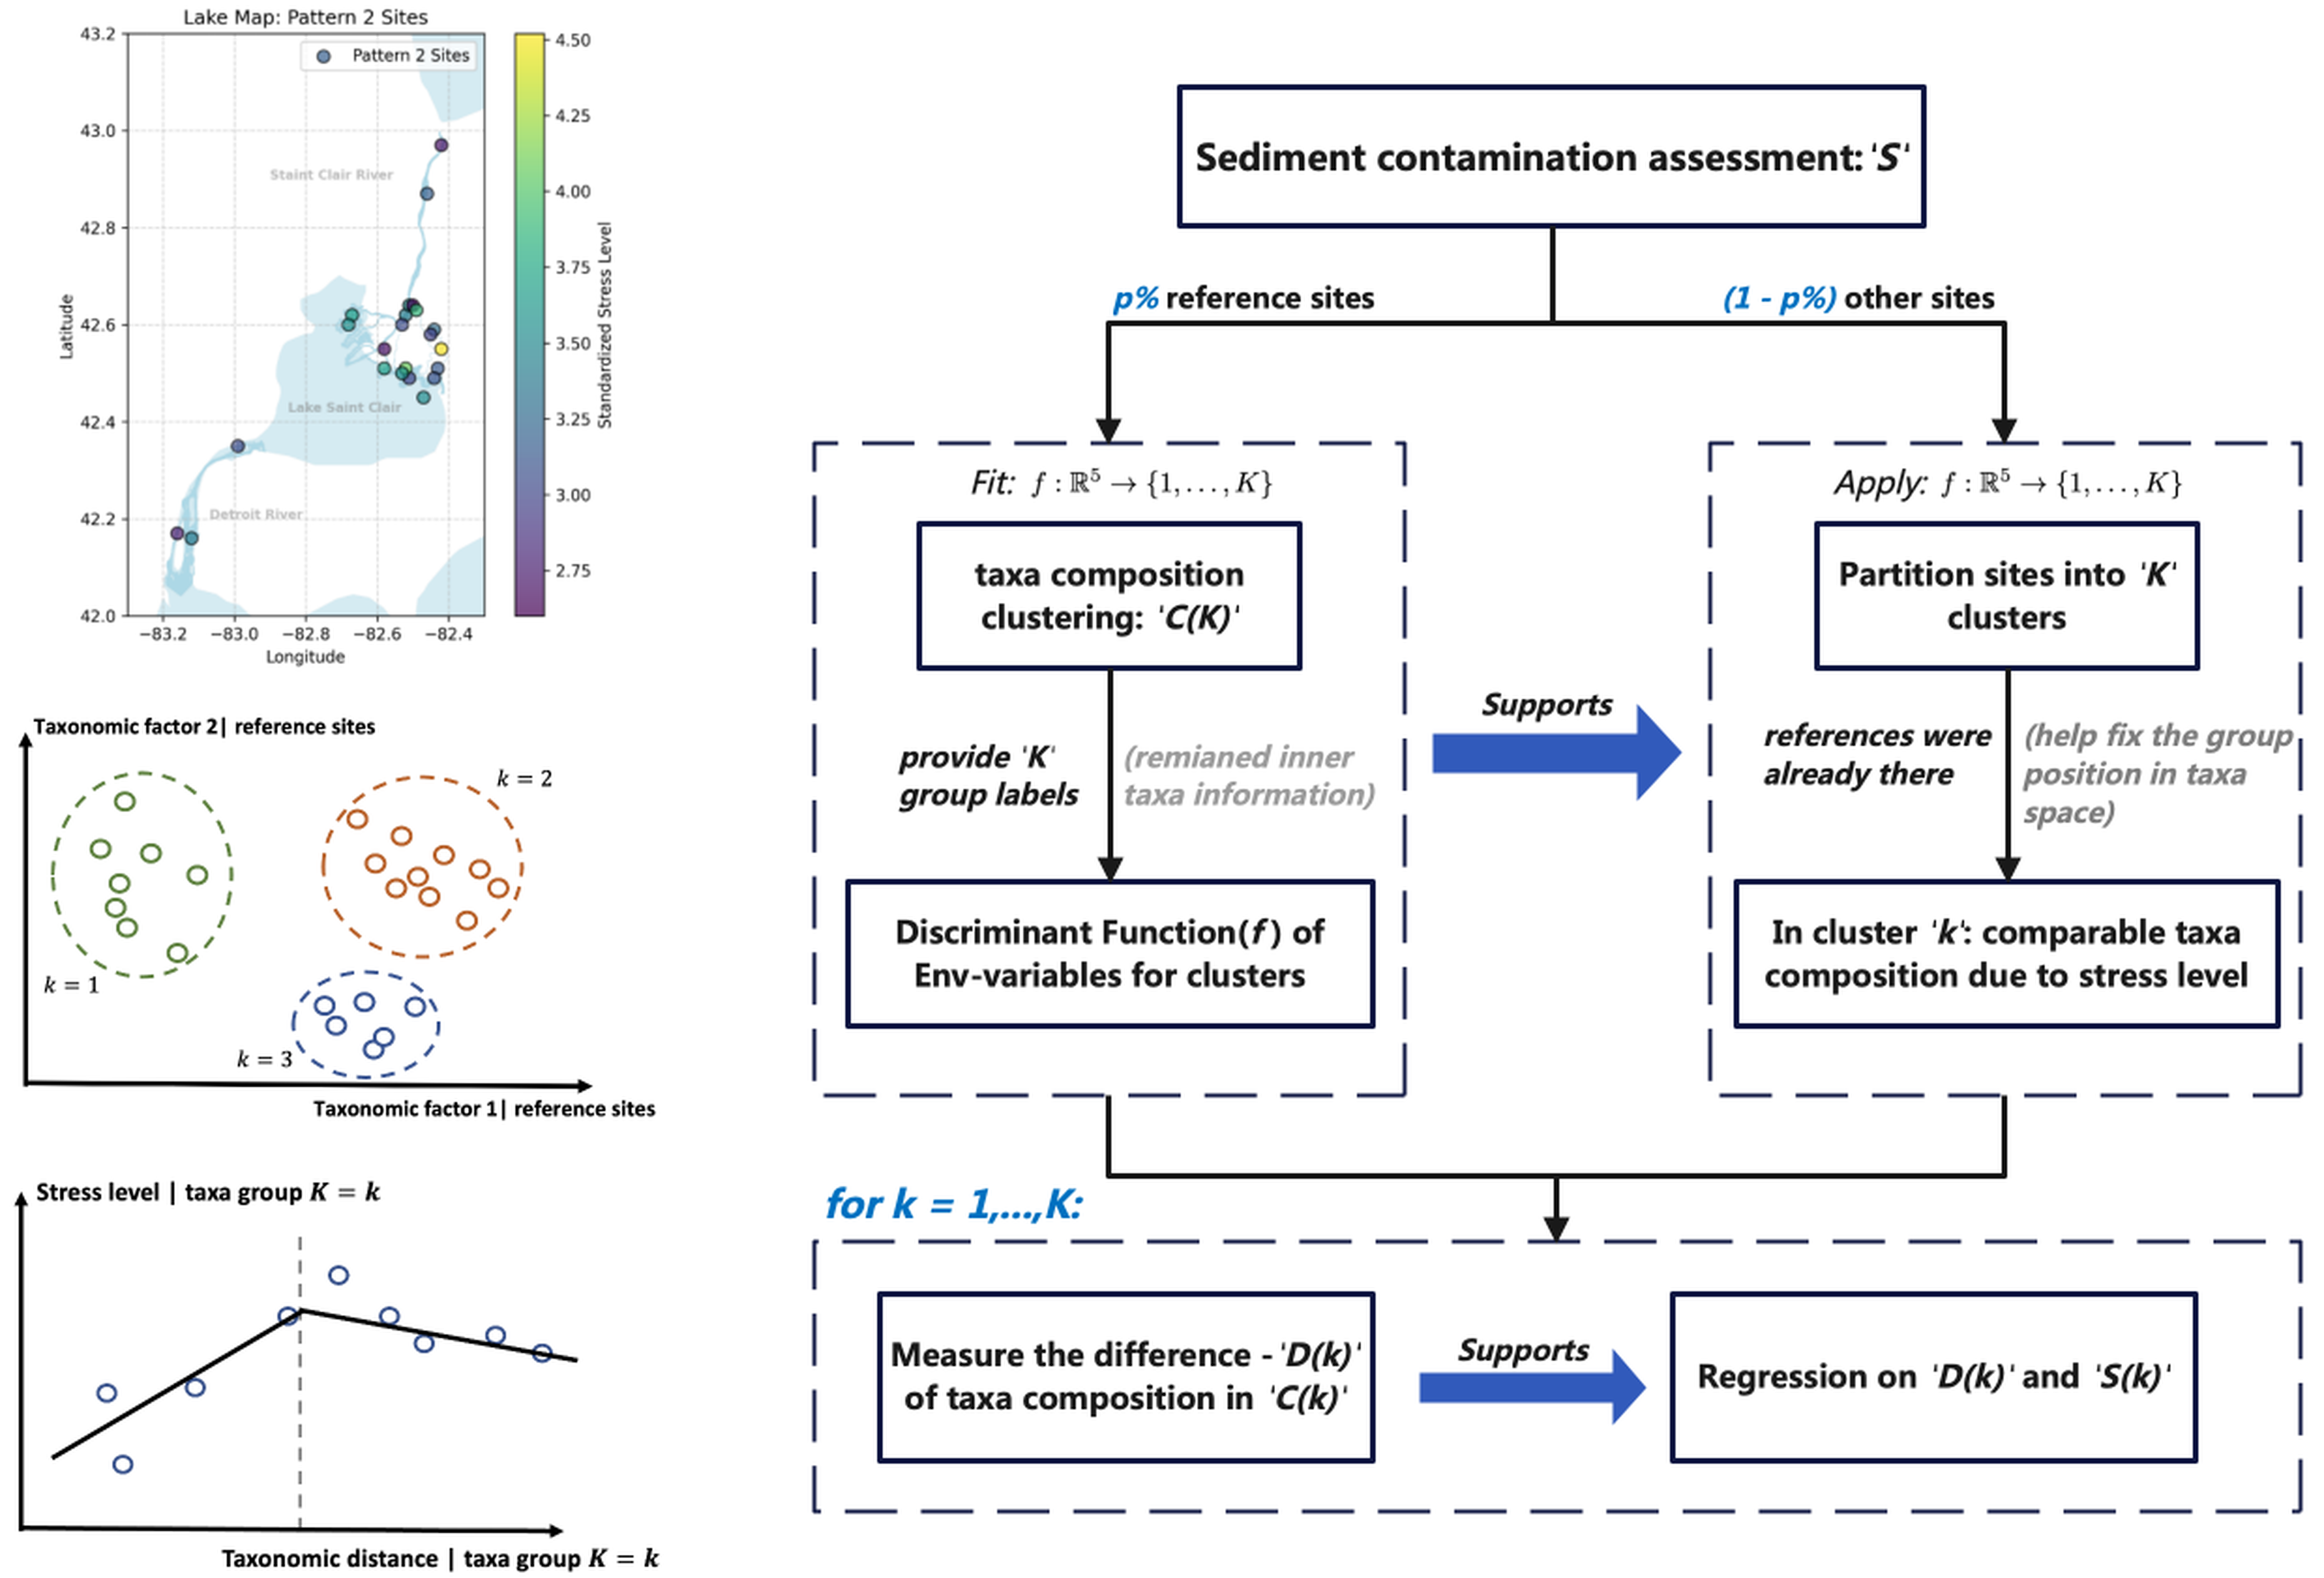
\includegraphics[width=\textwidth]{../results/workflow_of_general_workframe_part1.png}
%         \vspace{0.5em}
%         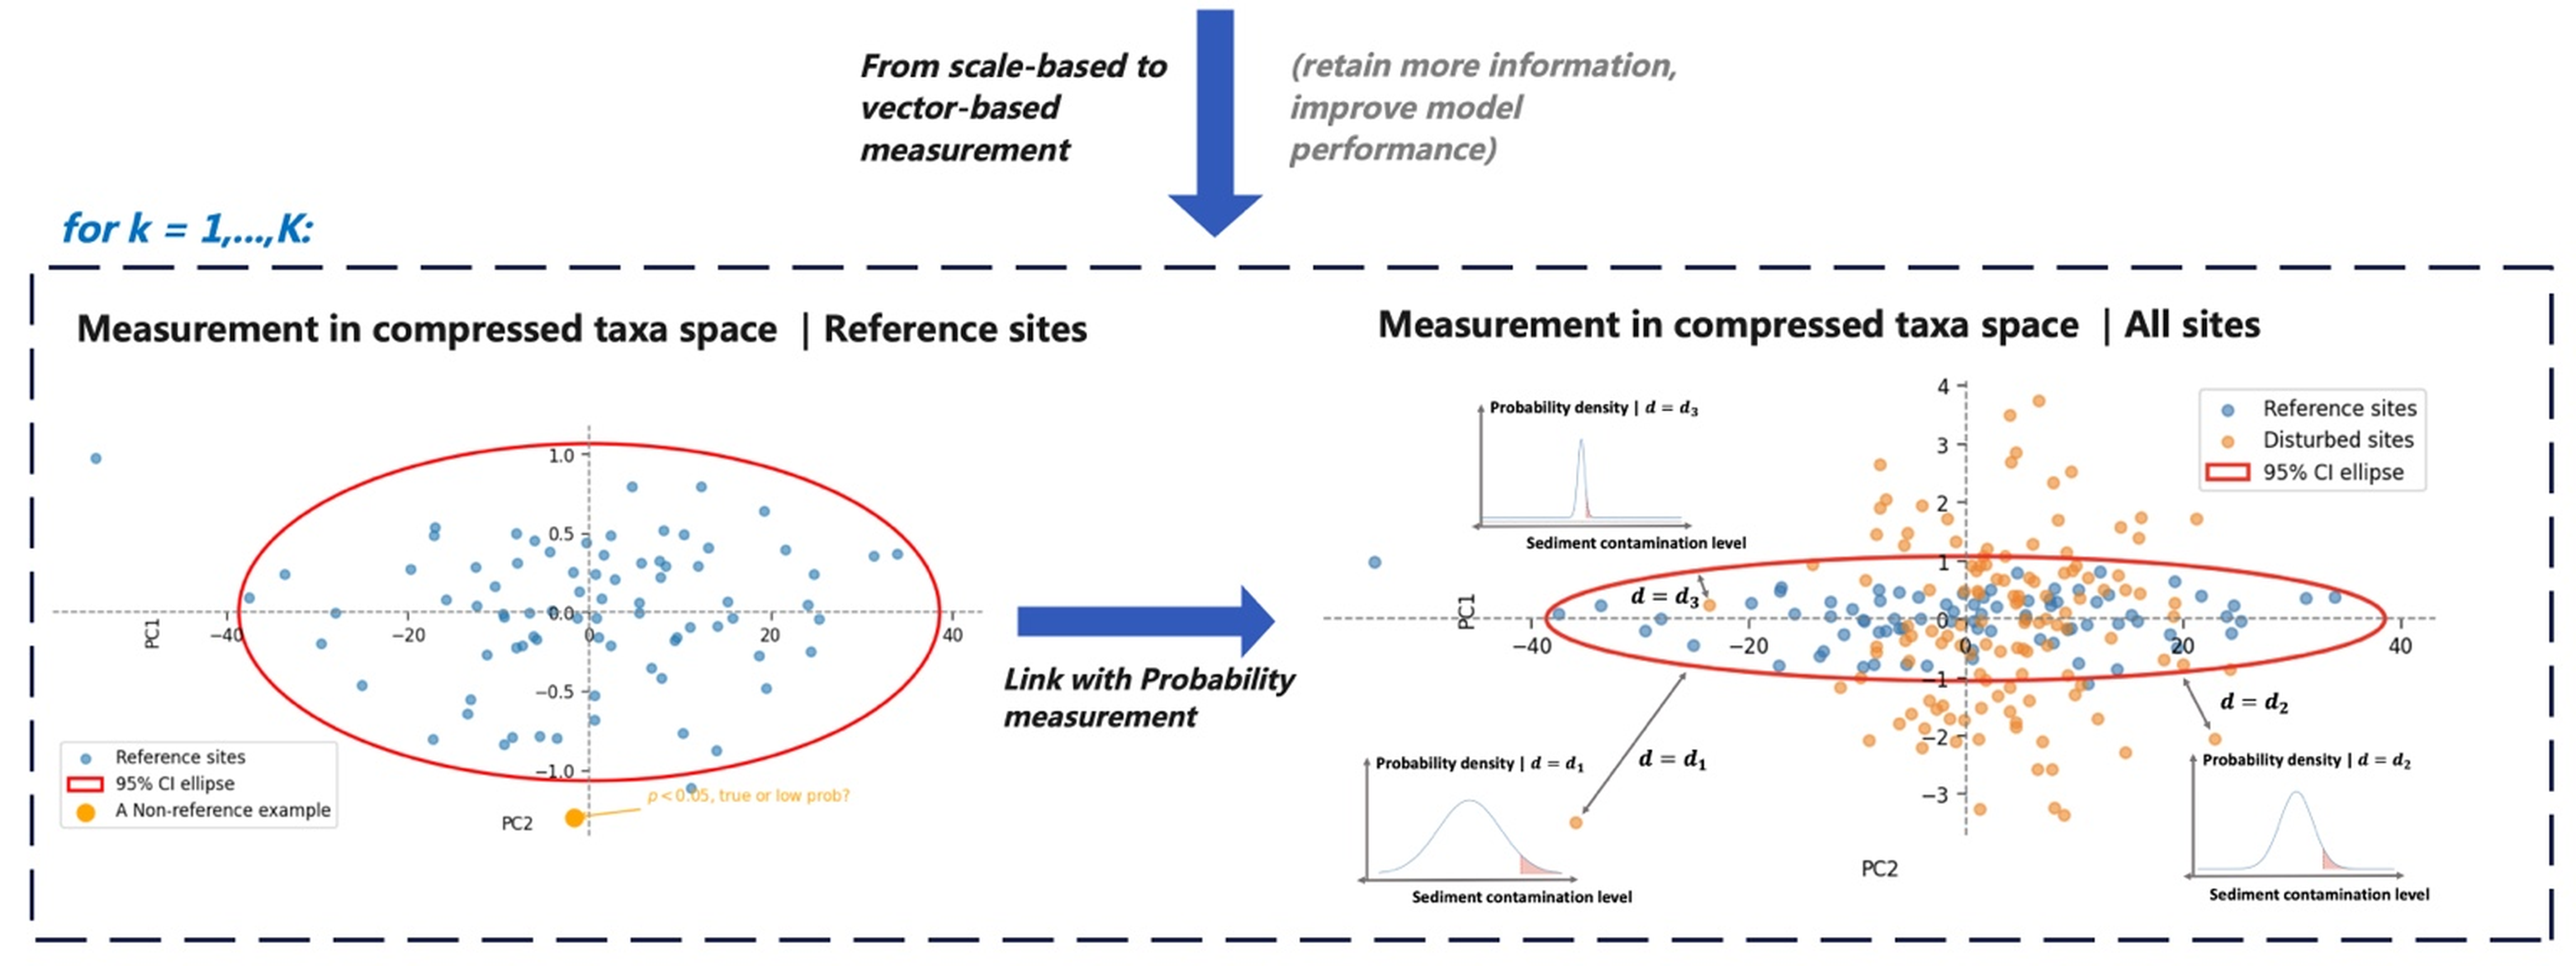
\includegraphics[width=\textwidth]{../results/workflow_of_general_workframe_part2.png}
%     \end{minipage}
%     \caption{Overview of workflow for the proposed methodology.}
%     \label{fig:workflow_of_general_workframe_parts}
% \end{figure}
\begin{figure}
\centering
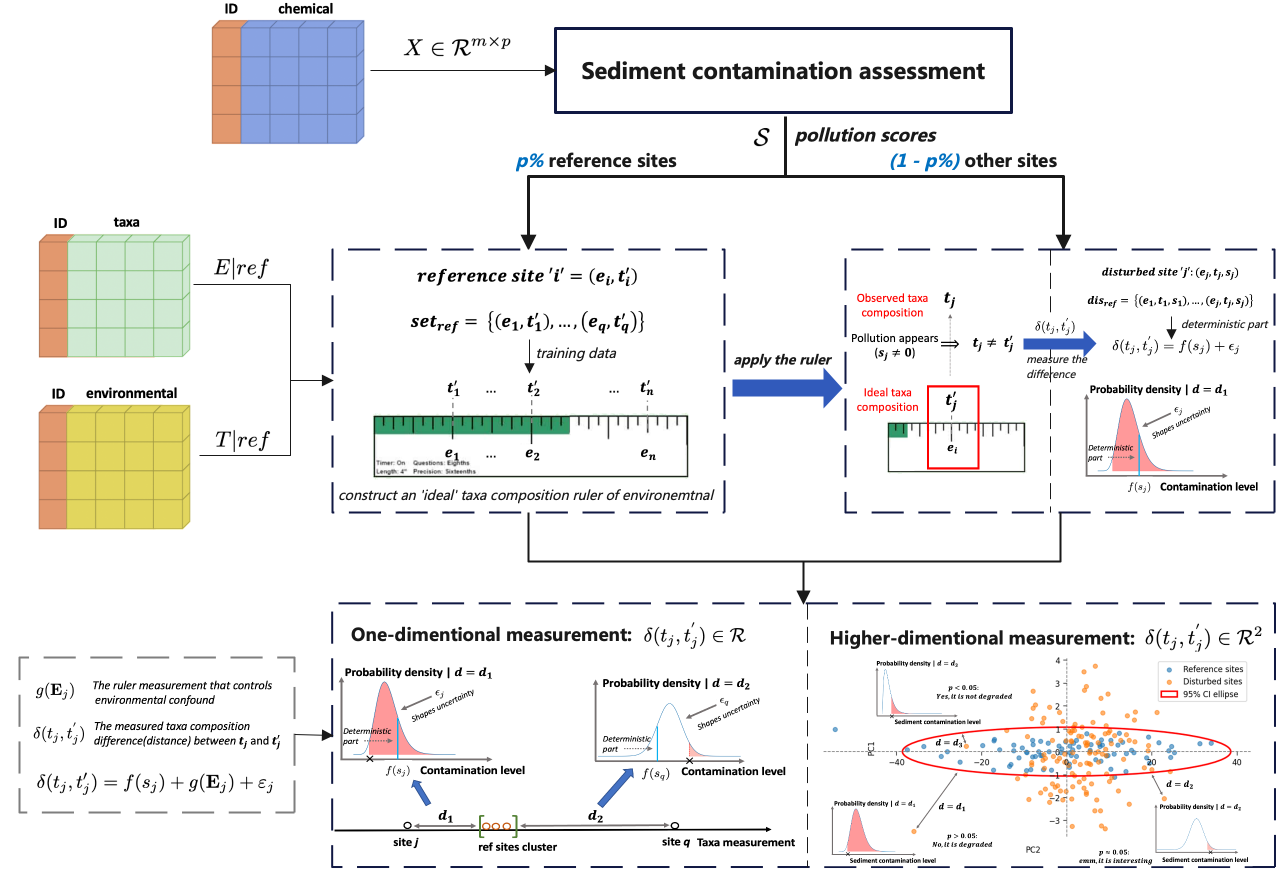
\includegraphics[width=0.8\textwidth]{../results/ideas_visualization/overall_framework.png}  
\caption{\textit{Overview of workflow for the proposed methodology.}}
\end{figure}
\subsection{Find Reference Sites - Sediment Contamination Assessment}

\begin{tcolorbox}[colback=white!95!gray, colframe=white!20!orange, 
    title = \textbf{External Reference: Data-driven PCA-based Pollution Assessment}]
    Detailed methodology for sediment contamination assessment has been developed separately.
    The method report that is under development is available at:
    \begin{itemize}
        \item \href{https://drive.google.com/file/d/1L43eq924ydxNeLgRYH4EsfJd8nvNVOf9/view}
        {Click to access: Method report draft}
    \end{itemize}
\end{tcolorbox}


To assess the sediment contamination and find the reference sites, we need to compute a composite stressor score \(s\) based on the chemical data.

Let \(m\) be the number of sampled sites and \(X \in \mathbb{R}^{m \times 30}\) denote the matrix of chemical element concentrations (each row represents a site and each column represents an element).
Doing a principal component analysis (PCA) on \(X\) transforms it into a set of uncorrelated and high variation-loading components \(Z\).
On top of the \(Z\), we can select \(k\)(\(< 30\)) proper components with defined criteria to cover the most variation in pollutant elements
and define a composite stressor score \(s \in \mathbb{R}^{m}\)
by summing or weighting the selected raw principal components or their normalised variants:


\begin{enumerate}
    \item \textbf{Principal component reduction} – Apply principal component analysis (PCA) to \(X\).  PCA transforms \(X\) into a set of uncorrelated components \(Z = X W\), where \(W \in \mathbb{R}^{30\times k}\) holds loadings of the first \(k\) principal components.

    \item \textbf{Composite stress score} – Let \(Z = [\,z_1,\dots,z_k\,]\) with \(z_i \in \mathbb{R}^{m}\) the vector of scores on the \(i\)-th principal component. 
     Define a composite stressor score \(s \in \mathbb{R}^{m}\) by summing or weighting the selected raw principal components:
    \[
    s_j \;=\;\sum_{i=1}^k \omega_i\,z_{i,j}, \quad j \in \{1,\dots,m\}
    \]
    where \(z_{i,j}\) is the \(i\)-th PC score at site \(j\) and \(\omega_i\) are predetermined weights (often set to 1 when components contribute equally).
\end{enumerate}

After computing the composite stressor score, we can add this new information to the originally compound matrix:
\[
\left[
\begin{array}{cccc}
X & E & T & s
\end{array}
\right] 
\in
\mathbb{R}^{m \times (51 + 1)}
\]

This \(s\) vector is used to rank the sites with respect to 
the stress level and filter the pristine reference sites where
human impact is minimal or absent. 
Specifically, we rank sites by \(s\) and retain the least‑stressed \(p\%\) of the sites,
create an indicator vector \(I_{\text{ref}} \in \mathbb{R}^{m}\) where \(I_{\text{ref},j} = 1\) if site \(j\) is a reference site and \(I_{\text{ref},j} = 0\) otherwise.
\[
\left[
\begin{array}{ccccc}
X & E & T & s & I_{\text{ref}}
\end{array}
\right] 
\in
\mathbb{R}^{m \times (52 + 1)}
\]
To this sites with \(I_{\text{ref},j} = 1\), we assume they represent
the ideal taxa composition that is shaped by the given environmental conditions,
supported by the minimal or absent human disturbance.
\[
\left[
\begin{array}{ccccc}
X & E & T & s & I_{\text{ref}} 
\end{array}
\right]_{I_{\text{ref}} = 1}
\in
\mathbb{R}^{(p\% \times m) \times (53)}
\]
Therefore, in this submatrix, the \(X\) matrix only contains the minimal \(p\%\) stress levels across all sites,
controlling the human disturbance on the taxa composition.

\begin{figure}[!h]
\centering
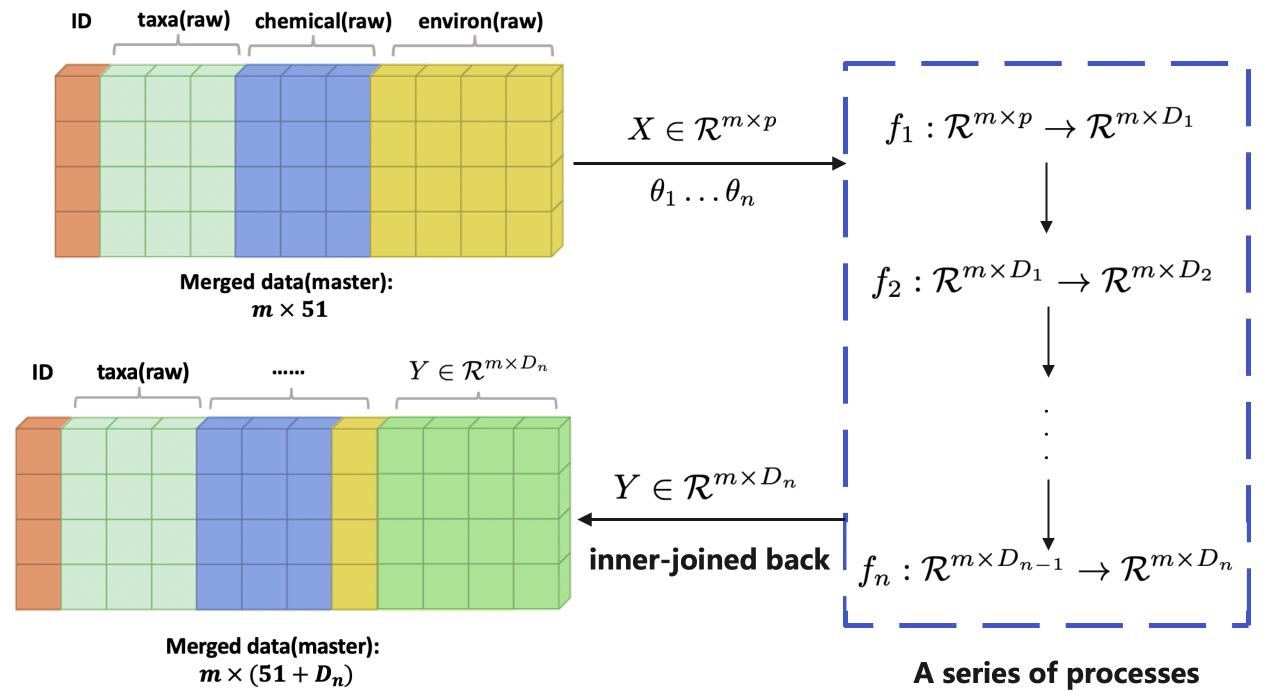
\includegraphics[width=0.8\textwidth]{../results/ideas_visualization/operate_data_throughout2.png}
\caption{\textit{Visualization of how the new information is generated and integrated into the existing matrix.}}
\label{fig:p4_rules_for_data_operation}
\end{figure}

\subsection{Prepare metrics of “ideal” taxa composition - Cluster Analysis on References}
In the matrix
$\left[
\begin{array}{ccccc}
X & E & T & s & I_{\text{ref}} 
\end{array}
\right]_{I_{\text{ref}} = 1}
$, the set of taxa composition \(T_{\text{ref}}\) 
is assumed to be shaped by the environmental variables \(E_{\text{ref}}\),
a well-fitted regression model between the \(E_{\text{ref}}\) and \(T_{\text{ref}}\)
matrices can numerically tell us how the taxa composition is multidimensionally shaped by the environmental variables.

However, considering that the \(E_{\text{ref}} \in \mathbb{R}^{(p\% \times m) \times 5}\) only provides 5 environmental variables,
and there are many other potentially unmeasured and unmeasurable environmental factors, it is nearly impossible to train a fully quantitative
inference model that describes the below relationship well:
\[
\mathcal{F} : E_{\text{ref}}^{(p\% \times m) \times 5} \to T_{\text{ref}}^{(p\% \times m) \times 16}, \quad \text{poorly fitted model}
\]

To solve this issue, we can construct constrained predicted values \(T_{\text{ref}}^{q} (q < 16)\) from the \(T_{\text{ref}}\) matrix, which 
provides limited yet information about the community structure, so that the model $\mathcal{F} : E_{\text{ref}}^{(p\% \times m) \times 5} \to T_{\text{ref}}^{(p\% \times m) \times q}$
can be trained to avoid overfitting and improve its prediction performance.
\[
\mathcal{F} : E_{\text{ref}}^{(p\% \times m) \times 5} \to T_{\text{ref}}^{(p\% \times m) \times q}, \quad \text{improved fitted model}
\]
One ideal way to do this information compression is 
to partition the reference sites into \(K\) different groups via clustering methods.

\[
T_{\text{ref}}^{(p\% \times m) \times q} = \mathcal{C}_K^{(p\% \times m) \times 1}  = clustering(T_{\text{ref}}^{(p\% \times m) \times 16}), \quad \text{where } q = 1
\]

By the clustering analysis and merging the resulting information into the reference-base matrix, the reference-base matrix can be updated as:
\[
\left[
\begin{array}{cccccc}
X & E & T & s & I_{\text{ref}} & \mathcal{C}_K
\end{array}
\right]_{I_{\text{ref}} = 1}
\in
\mathbb{R}^{(p\% \times m) \times (53 + 1)}
\]


Even though the \(C_K\) is computed from the clustering analysis on taxa composition matrix \(T_{\text{ref}}\),
the underlying environmental conditions(\(E_{\text{ref}}\)) are the actual drivers to lead to the clustering results,
based on the fundamental assumption that "the reference taxa-composition is shaped by the environmental conditions".

\begin{figure}[!h]
    \centering
    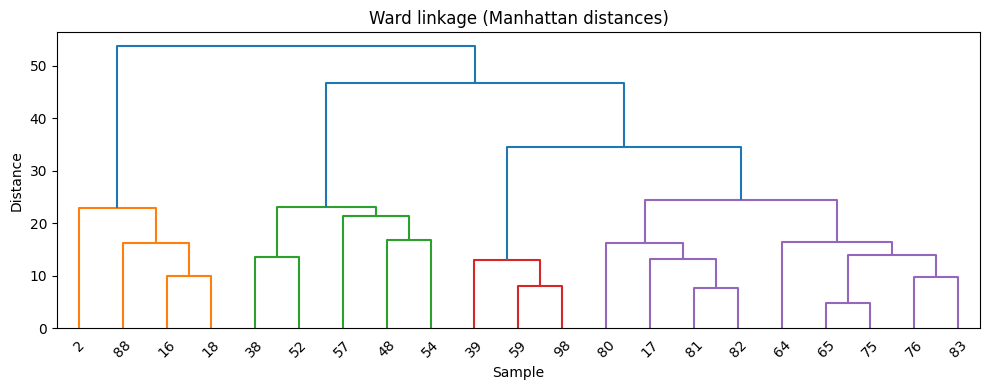
\includegraphics[width=0.8\textwidth]{../presentation/figures/p10_clustering_results.png}
    \caption{\textit{An example of hierarchical clustering results on the taxa composition matrix of the references
    with selected clustering number \(K\).}}
    \label{fig:p10_clustering_results}
\end{figure}


\subsection{Construct “ideal” taxa composition ruler of environmental factors - Fit a Discriminant Function}

\begin{figure}[!h]
\centering
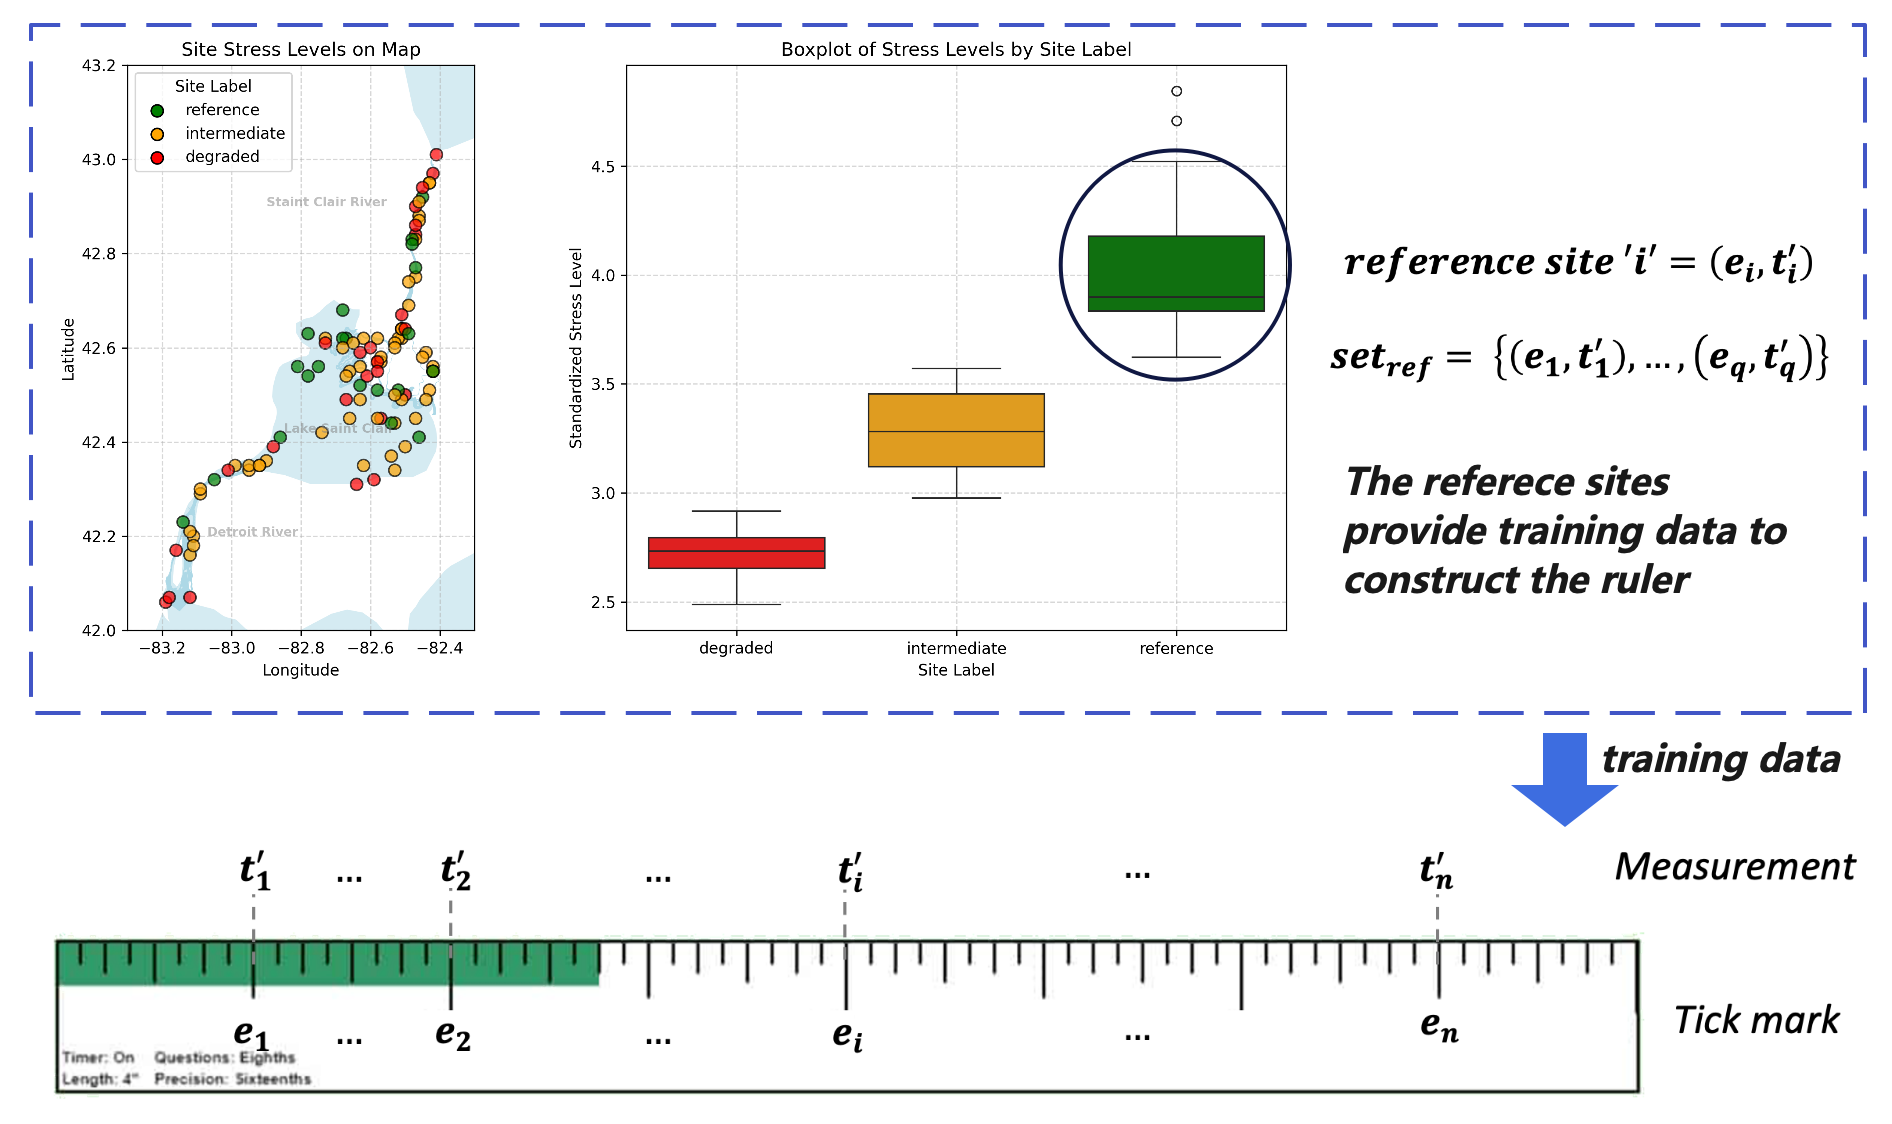
\includegraphics[width=0.8\textwidth]{../results/ideas_visualization/constructing_ruler.png}
\caption{\textit{The reference sites are used as training data to construct this 'ideal' taxa composition ruler.
($t^{'}_{j}$ represents the raw taxa composition of site \(j\), it has not been transformed into the cluster label \(\mathcal{C}_K\) yet.)}}
\label{fig:constructing_ruler}
\end{figure}

At this stage, there are constrained taxa composition information - cluster labels \(\mathcal{C}_K\) that can be used as
response variables in training the environmental-taxa composition regression. 
Specifically, a discriminant function can be fitted here:
\[
\mathcal{F_{\text{dis}}} : E_{\text{ref}}^{(p\% \times m) \times 5} \to \mathcal{C}_K^{(p\% \times m) \times 1}
\]

This discriminant function \(\mathcal{F_{\text{dis}}}\) fitted on the reference sites tells us how the environmental variables - \(E\) roughly shape the 
taxa composition by assigning each site to one of the taxa composition groups \(\mathcal{C}_K\).

During the training stage, the reference sites are partitioned into the \(K\) taxa composition groups, 
helping to fix the group positions in taxa composition space with the pristine taxa composition part in 
each group. \textbf{However, it does not mean there is only pristine taxa composition in each cluster.
When human disturbance appears, the pristine taxa composition should be shifted to a new position in the taxa composition space,
which is how the disturbed sites look like in the same taxa composition space.}

Therefore, these reference sites are partitioned (by clustering) into different clusters to play the role of 'ideal' metrics
on a ruler of taxa composition (by discriminant function), this ruler measures the 'ideal' taxa composition structure that a site should have given its environmental conditions.

An imaginable scenario is that, when we use the fitted \(\mathcal{F_{\text{dis}}}\) as a ruler to measure the taxa composition of sites that are affected by human disturbance,
the measured 'ideal' taxa composition is not equal to the truly observed taxa composition. 
And this difference in taxa composition is caused by the human disturbance, which was measured by the sediment contamination assessment in the previous step.

\subsection{Mark the “ideal taxa composition” for disturbed sites - Apply the Discriminant Function}

Given the fitted discriminant function \(\mathcal{F_{\text{dis}}}\), we can classify the rest \(1 - p\%\) of the sites
into the taxa composition groups, where reference sites with similar environmental conditions are already assigned into.

Because the clustering analysis was done on the reference sites, the known information on the disturbed sites should look like:
\[
\left[
\begin{array}{ccccc}
X & E & T & s & I_{\text{ref}}
\end{array}
\right]_{I_{\text{ref}} = 0}
\in
\mathbb{R}^{((1 - p\%) \times m) \times (53)}
\]

After applying the discriminant function on these disturbed sites, 
we can know their environmental-deterministic taxa composition groups,
\(\mathcal{C}_K^{((1 - p\%) \times m) \times 1}\).
It expands the disturbed-base matrix to:
\[\left[
\begin{array}{cccccc}
X & E & T & s & I_{\text{ref}} & \mathcal{\hat C}_K
\end{array}
\right]_{I_{\text{ref}} = 0}
\in
\mathbb{R}^{((1 - p\%) \times m) \times (53 + 1)}
\]

Compare it with the reference-base matrix,
we can see that the sites having the same taxa composition cluster \(\mathcal{C}_K\) are now comparable 
with the control of environmental variables \(E\).

To the \(i\) th site in the matrix:

\[\left[
\begin{array}{cccccc}
X & E & T & s & I_{\text{ref}} & \mathcal{C}_K
\end{array}
\right]_{I_{\text{ref}} = 1}
\in
\mathbb{R}^{(p\% \times m) \times (53 + 1)}
\]

If the site has \(\mathcal{C}_{K_i} = \mathcal{\hat C}_{K_j}\), then the \(i\)-th reference site is comparable with the disturbed site \(j\)-th site in the taxa composition space with the control of environmental conditions.
The difference in their taxa composition, \(\delta T_{i,j}\), is caused by the human disturbance, \(\delta X_{i,j}\), between the two sites.

\[
\mathcal{C}_{K_i} = \mathcal{\hat C}_{K_j} \Rightarrow E_{\text{ref}, i}^{(1 \times 5)} \approx E_{\text{dis}, j}^{(1 \times 5)} \Rightarrow \delta T_{i,j} = \mathcal{F}_{reg}(\delta X_{i,j})
\]

Therefore, the sites within the same taxa composition group will be used to fit the regression model - \(\delta T_{i,j} = \mathcal{F}_{reg, k}(\delta X_{i,j})\), 
and these completed groups can be found through
the merging-dismantle process of the two base matrices.

Merging the reference-base matrix and the disturbed-base matrix:
\[
\text{stack}\left(
\left[
\begin{array}{cccccc}
X & E & T & s & I_{\text{ref}} & \mathcal{C}_K
\end{array}
\right]_{I_{\text{ref}} = 1}
,
\left[
\begin{array}{cccccc}
X & E & T & s & I_{\text{ref}} & \mathcal{\hat C}_K
\end{array}
\right]_{I_{\text{ref}} = 0}
\right)
\]
\[
\Rightarrow
\left[
\begin{array}{cccccc}
X & E & T & s & I_{\text{ref}} & \mathcal{\hat C}_K
\end{array}
\right]
\]

Split the merged matrix into \(K\) submatrices, where each submatrix contains the same cluster label \(\mathcal{C}_k\):

\[
\left[
\begin{array}{cccccc}
X & E & T & s & I_{\text{ref}} & \mathcal{\hat C}_K
\end{array}
\right]
=
\left\{
\begin{array}{ll}
\left[
\begin{array}{cccccc}
X & E & T & s & I_{\text{ref}} & \mathcal{C}_1
\end{array}
\right] & \text{if } \mathcal{C}_K = 1 \\[1.2em]
\left[
\begin{array}{cccccc}
X & E & T & s & I_{\text{ref}} & \mathcal{C}_2
\end{array}
\right] & \text{if } \mathcal{C}_K = 2 \\[0.8em]
\quad\vdots & \quad
\vdots \\[0.8em]
\left[
\begin{array}{cccccc}
X & E & T & s & I_{\text{ref}} & \mathcal{C}_K
\end{array}
\right] & \text{if } \mathcal{C}_K = K
\end{array}
\right.
\]

Within each submatrix,
$
\left[
\begin{array}{cccccc}
X & E & T & s & I_{\text{ref}} & {\mathcal{C}_k}
\end{array}
\right]
$, we will numerically measure the difference in the taxa composition 
between the degraded sites and the reference sites,
$\delta T_k$, this distance in taxa composition will be explained by the 
relative stress level of each site, \(\delta X_k\).

\begin{figure}
\centering
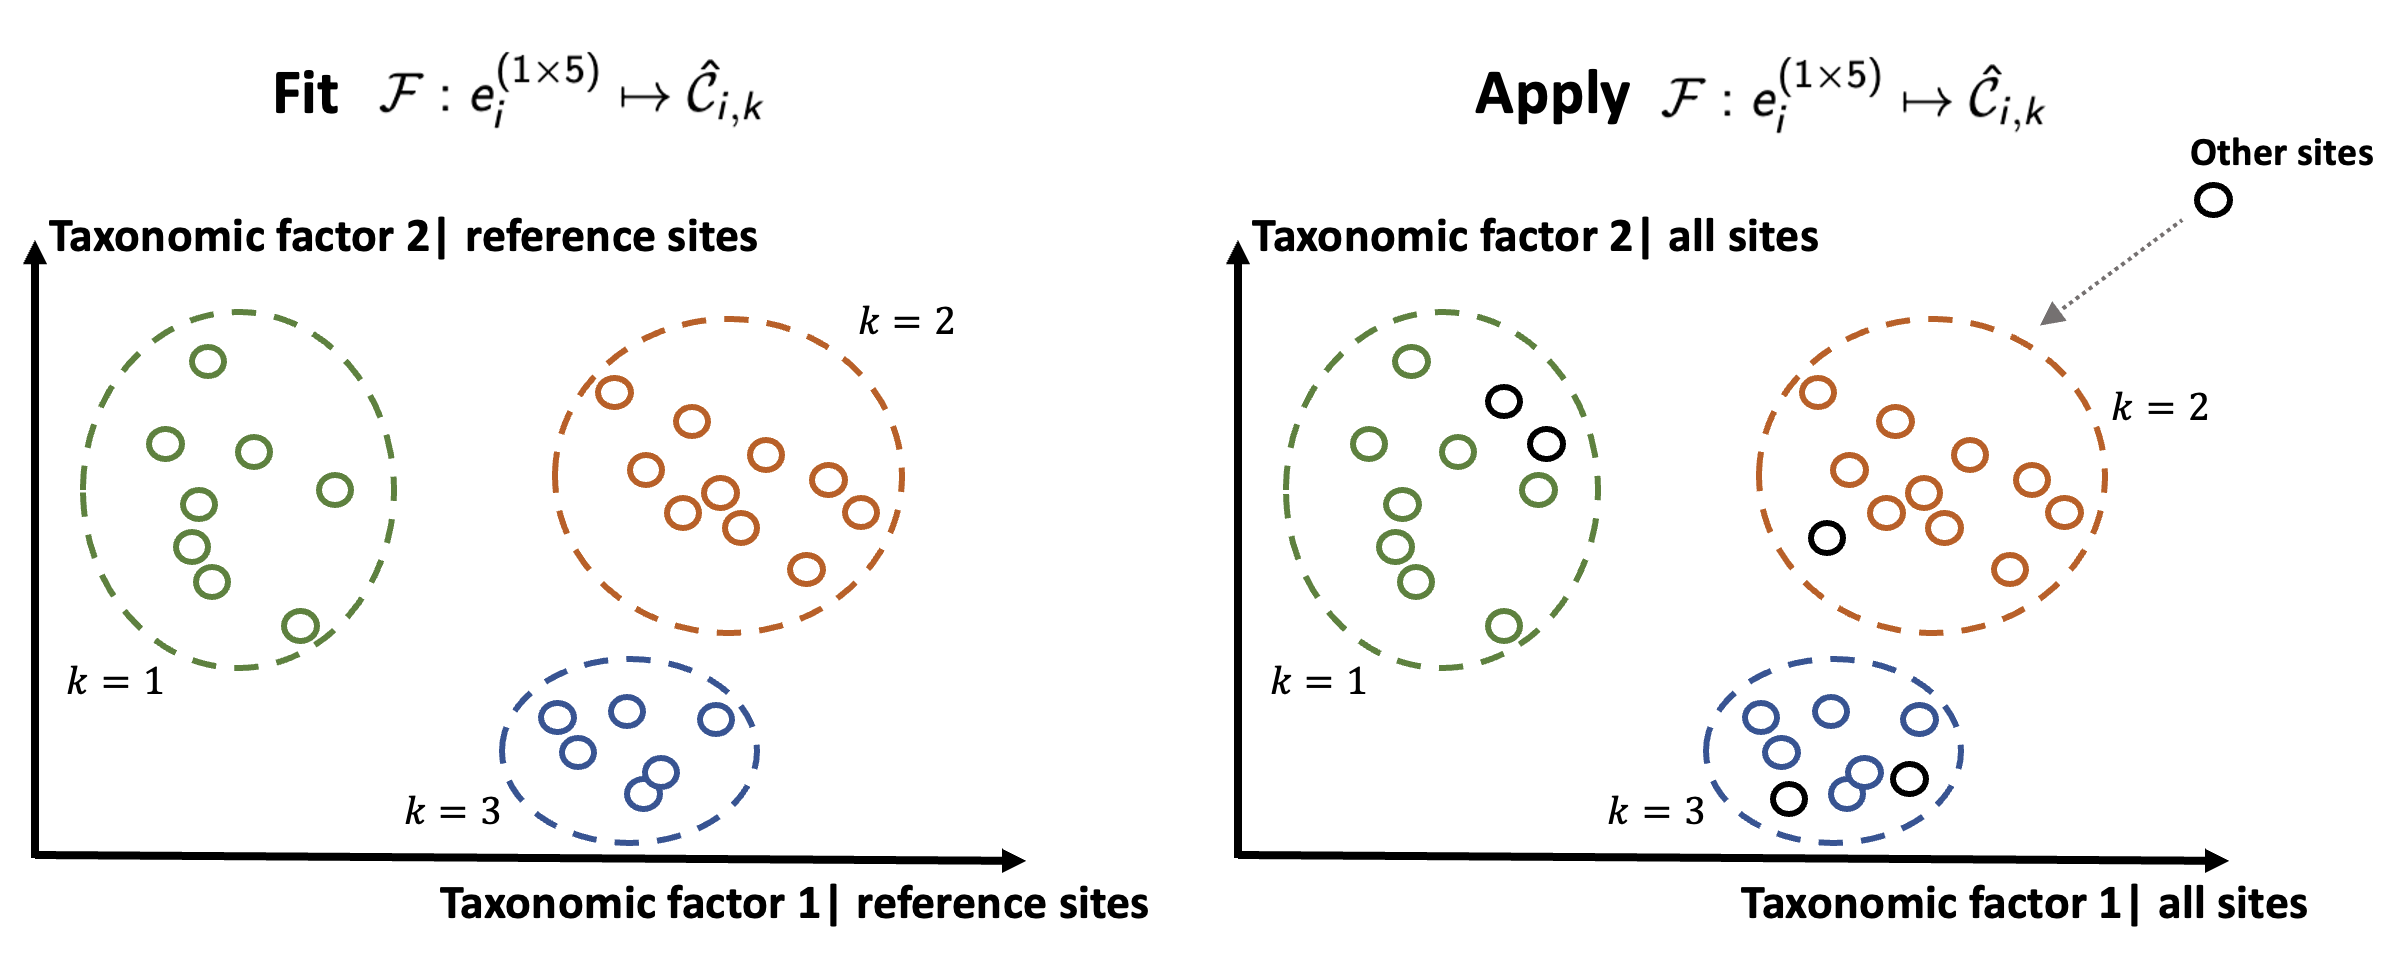
\includegraphics[width=0.8\textwidth]{../presentation/figures/p12_fit_apply_discriminant_function.png}
\caption{\textit{Visualization of the fitting and application of the discriminant function that assigns disturbed sites to the environmentally determined taxa composition groups.
}}
\label{fig:p12_fit_apply_discriminant_function}
\end{figure}

\subsection{Measure the difference from “pristine” to “true” taxa composition - Multivariate Gaussian Deviation Index }

\begin{figure}[!h]
    \centering
    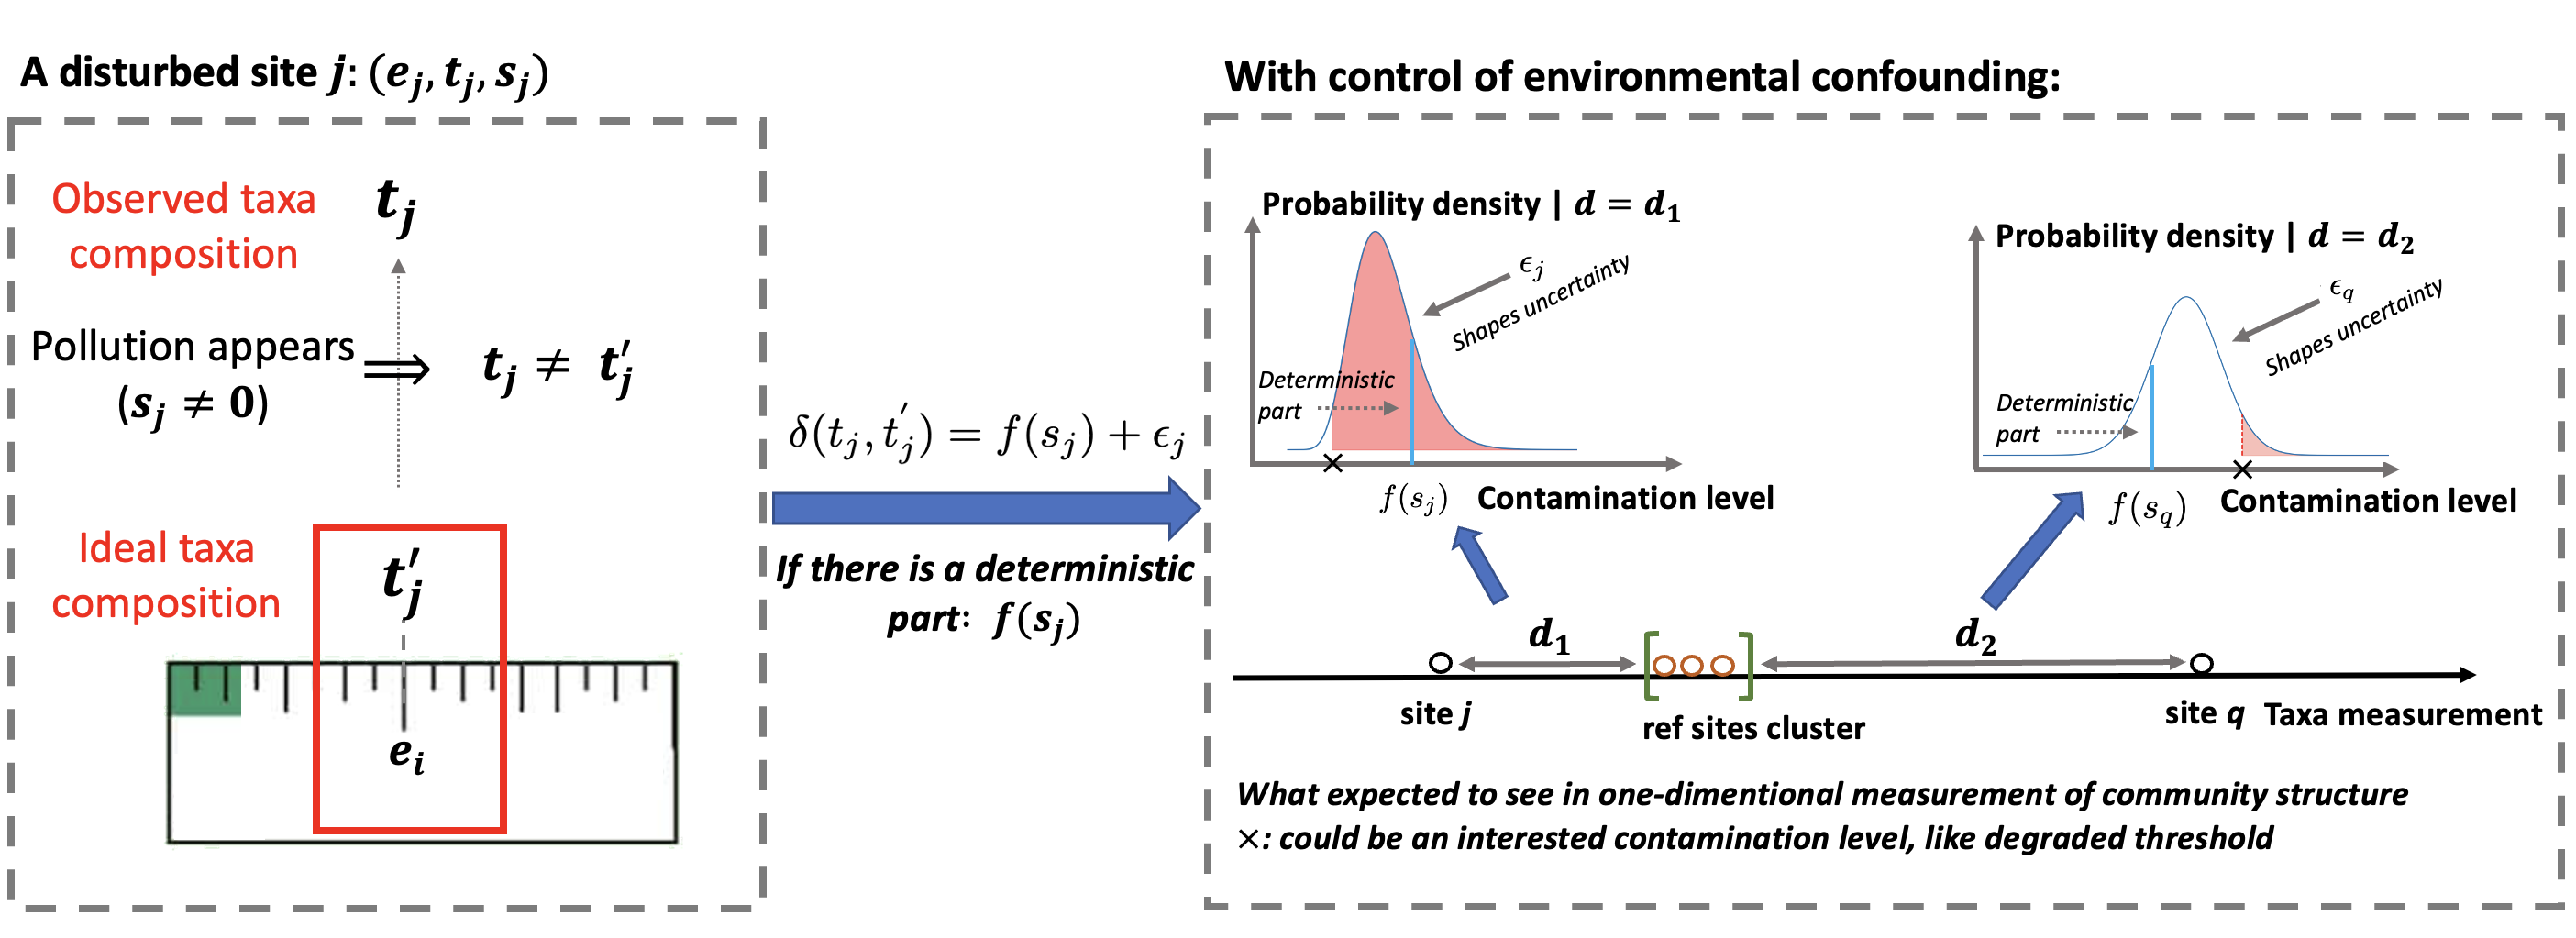
\includegraphics[width=0.8\textwidth]{../results/ideas_visualization/mark_taxa_difference_and_explain.png}
    \caption{\textit{The difference in taxa composition between the observed($t_{j}$) and ruler measured($t^{'}_{j}$) is connected to the sediment contamination level($s$).}}
    \label{fig:mark_taxa_difference_and_explain}
\end{figure}

Within each taxa-composition group $\mathcal{C}_k$, let $\mathcal{R}_k$ denote the set of reference sites ($I_{\text{ref}}=1$) and $\mathcal{D}_k$ the set of disturbed sites ($I_{\text{ref}}=0$).
We construct a site-level deviation metric that quantifies how far a site's observed community is from the pristine expectation of its group while controlling for environmental setting via $\mathcal{C}_k$.

% \paragraph{Choice of scale for community data.}
Because taxa compositions are multivariate and often compositional/zero-inflated, 
we first work on a transformed scale using the Hellinger transformation:
\[
\phi_{\mathrm{Hel}}:\;\mathbb{R}^{16}_{\ge 0}\rightarrow\mathbb{R}^{16}, \quad
\phi_{\mathrm{Hel}}(\mathbf{t})=
\left(
\sqrt{\frac{t^{(1)}}{\sum_{\ell=1}^{16} t^{(\ell)}}},\;
\dots,\;
\sqrt{\frac{t^{(16)}}{\sum_{\ell=1}^{16} t^{(\ell)}}}
\right).
\]
This transformation converts each taxon abundance to the square root of its relative abundance, 
reducing the influence of highly dominant taxa while preserving ecological distance relationships.
All subsequent quantities are computed on $\phi_{\mathrm{Hel}}(T)$; 
to simplify notation we overwrite $T \leftarrow \phi_{\mathrm{Hel}}(T)$.

There are other transformations that may be preferred depending on the context (e.g., log-ratio transforms, or raw counts),
the Hellinger transformation is tentative and can be replaced as needed.


After the transformation, for group $k$, compute the reference centroid and covariance
\[
\boldsymbol{\mu}_k \;=\; \frac{1}{|\mathcal{R}_k|}\sum_{i\in\mathcal{R}_k} T_{i}, 
\qquad
\boldsymbol{\Sigma}_k \;=\; \mathrm{Cov}\{T_{i}: i\in\mathcal{R}_k\} + \lambda I_{16},
\]
where $\lambda>0$ is a small ridge term to ensure invertibility and numerical stability, and 
$I_{16}$ is the $16\times 16$ identity matrix.
These parameters $(\boldsymbol{\mu}_k,\boldsymbol{\Sigma}_k)$ define a 
multivariate Gaussian-like distribution in the $16$-dimensional taxa space, representing the 
\emph{pristine community cloud} for group $k$.
Under this view, each reference site is a draw from 
$\mathcal{N}(\boldsymbol{\mu}_k, \boldsymbol{\Sigma}_k)$, 
and the geometric shape of this cloud is an ellipsoid whose orientation and size are determined by 
$\boldsymbol{\Sigma}_k$.

\subsubsection{Value-based Measurement: Z-score Community Index (ZCI)}
For any site $j$ in group $k$ (reference or disturbed), define the multivariate standardized 
deviation from the pristine centroid as the Mahalanobis distance:
\[
\mathrm{ZCI}_{k,j} \;=\; \sqrt{\big(T_{j}-\boldsymbol{\mu}_k\big)^{\top}\,\boldsymbol{\Sigma}_k^{-1}\,\big(T_{j}-\boldsymbol{\mu}_k\big)}.
\]
This measures how far $T_j$ lies from the center of the pristine Gaussian cloud, in units that 
account for both taxon-specific variability and cross-taxon correlations.
It effectively reduces the $16$-dimensional deviation vector to a \emph{single scalar score} 
while preserving the anisotropic geometry of the reference distribution.

When a diagonal approximation is preferred, use the ``sum of squared z-scores'' variant:
\[
\mathrm{ZCI}^{(\mathrm{diag})}_{k,j} \;=\; \sqrt{\sum_{\ell=1}^{16}\left(\frac{T^{(\ell)}_{j}-\mu^{(\ell)}_{k}}{\sigma^{(\ell)}_{k}}\right)^{2}},
\]
where $\sigma^{(\ell)}_{k}$ is the reference standard deviation of taxon $\ell$ in group $k$ 
(robust alternatives such as median absolute deviation may also be used).
This ignores inter-taxon correlations, treating the pristine cloud as an axis-aligned hypersphere, 
which can be more stable when the number of reference sites is small relative to the number of taxa.

\begin{figure}[!h]
\centering
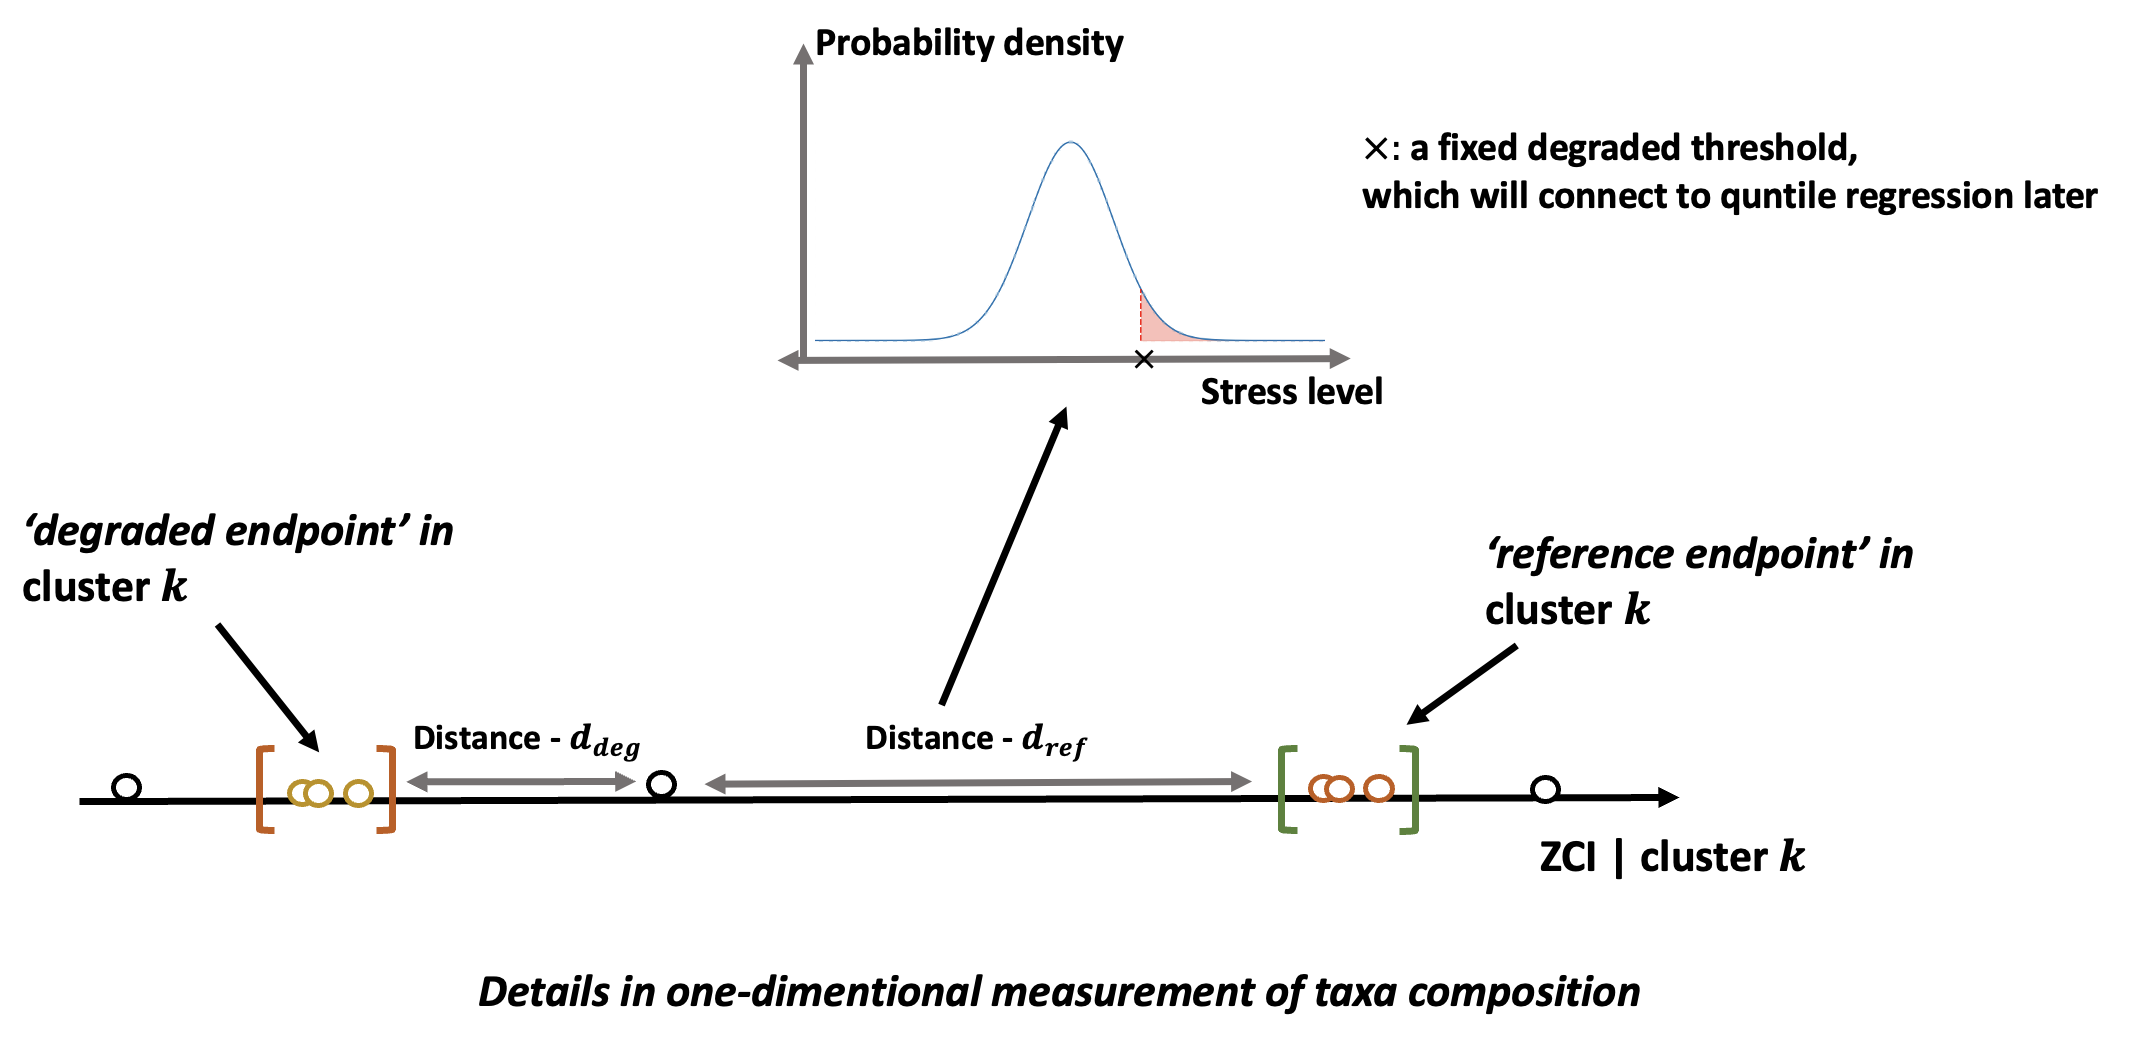
\includegraphics[width=0.8\textwidth]{../presentation/figures/p15_details_of_taxa_difference_in_1dimention.png}
\caption{\textit{Visualization of the details of taxa community structure differences measured in one-dimensional ZCI.}}
\label{fig:p15_details_of_taxa_difference_in_1dimention}
\end{figure}

\subsubsection{Vector-based Measurement: multi-dimensional ZCI}
The scalar $\mathrm{ZCI}_{k,j}$ summarizes deviation magnitude but discards the 
\emph{direction} of change in community composition.  
To retain more structure, the same Gaussian framework can be used to construct a 
multi-dimensional ZCI:

\begin{enumerate}
    \item \textbf{Whitening of deviations
    \footnote{Whitening means: Centering (subtracting \(\mu_k\)), rescaling and rotating so that the reference
    covariance becomes the identity matrix. Knowing that \(\Sigma_k = \frac{1}{|T|-1} (T - \mu)^T (T - \mu)\),
    replacing the \(T\) with \(\tilde{T} = \Sigma_k^{-1/2} (T - \mu)\),
    the new covariance matrix \(\tilde \Sigma_k\) becomes \(\frac{1}{|\tilde T| - 1} (\tilde{T} - \tilde \mu)^T (\tilde{T} - \tilde \mu) = I \) 
    . Here, \(T\) and \(\mu\) are both matrices and \(\Sigma_k\) is a non-singular matrix.}
    :} For each site $j$ in group $k$, compute the whitened deviation vector
    \[
    \tilde{T}_{k,j} = \boldsymbol{\Sigma}_k^{-1/2} (T_j - \boldsymbol{\mu}_k),
    \]
    where $\boldsymbol{\mu}_k$ and $\boldsymbol{\Sigma}_k$ are estimated from the reference sites.  
    Denote the matrix of whitened deviations for \emph{reference} sites as 
    $\tilde{T}_{k,\mathrm{ref}} \in \mathbb{R}^{n_{\mathrm{ref},k} \times 16}$.  
    In this whitened space, the reference cloud is isotropic and centered at the origin.
    
    \item \textbf{PCA fitted on whitened reference sites:}  
    Perform principal component analysis (PCA) on $\tilde{T}_{k,\mathrm{ref}}$ to obtain the loading matrix $V_k$.  
    Retain the first $d$ principal axes $V_{k,(1:d)}$, where $d=2$ gives a two-dimensional ZCI.

    \item \textbf{PCA applied to disturbed sites:}  
    For each disturbed site $j$, compute its whitened deviation $\tilde{T}_{k,j}$ using the \emph{same} $\boldsymbol{\mu}_k$ and $\boldsymbol{\Sigma}_k^{-1/2}$ from the reference sites, and project it onto the retained principal axes:
    \[
    \big( \mathrm{ZCI}^{(1)}_{k,j}, \mathrm{ZCI}^{(2)}_{k,j} \big)
    = \tilde{T}_{k,j} \; V_{k,(1:2)}.
    \]
\end{enumerate}

These coordinates preserve both magnitude and orientation of deviation in the most informative 
subspace of the pristine community cloud, enabling more nuanced comparisons between sites 
that have similar scalar ZCI values but differ in the \emph{type} of community shift.  
The scalar $\mathrm{ZCI}_{k,j}$ can be recovered as the Euclidean norm of these coordinates.

\begin{figure}[!h]
\centering
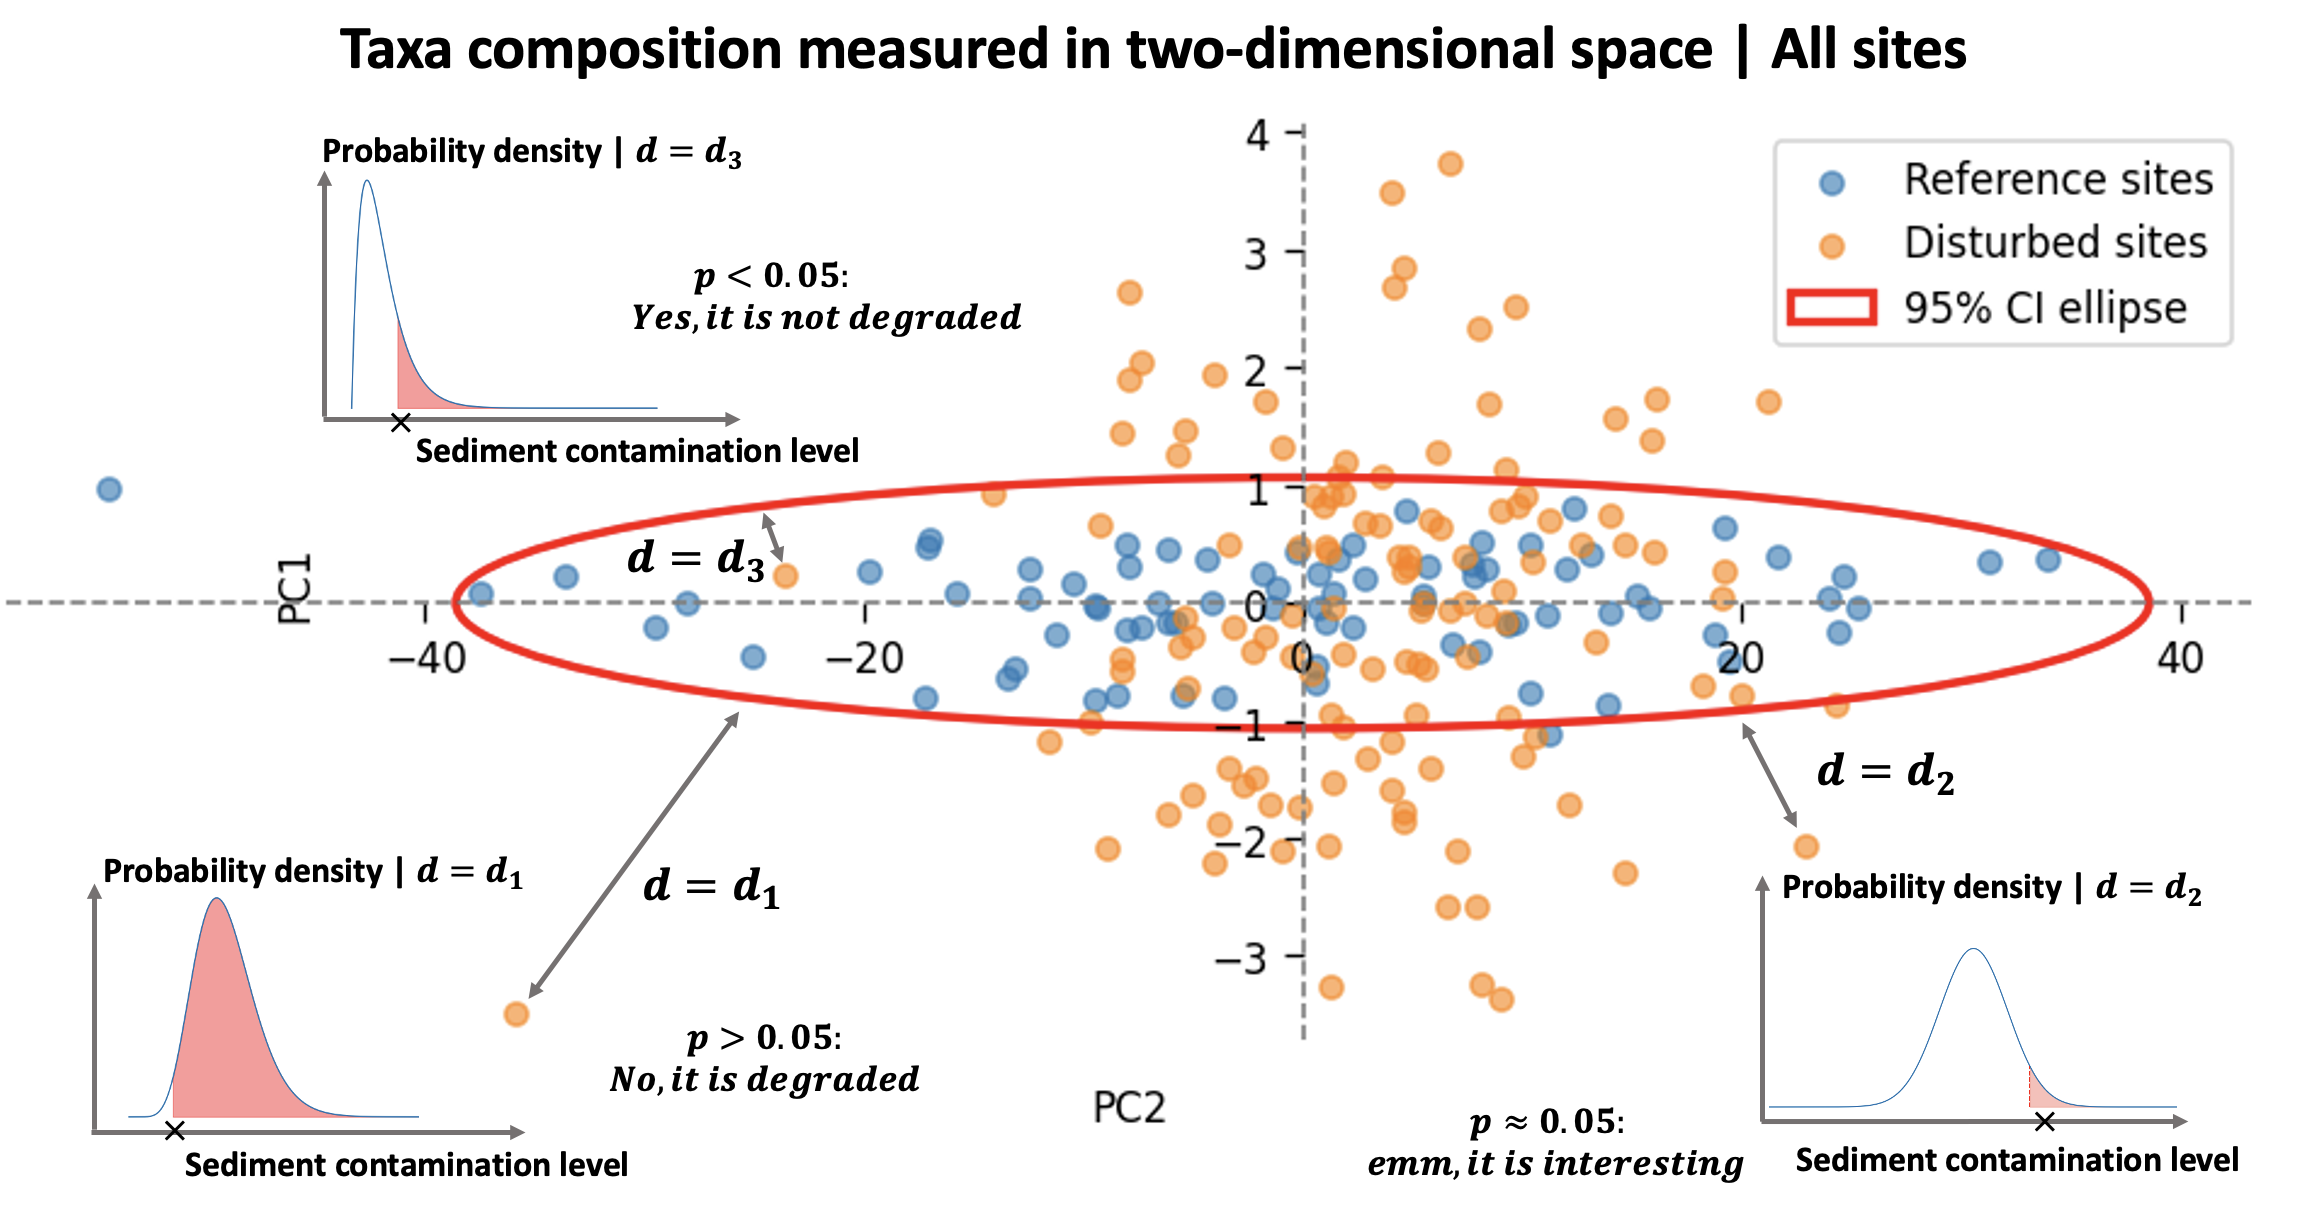
\includegraphics[width=0.8\textwidth]{../presentation/figures/p18_all_sites_in_2dimensional.png}
\caption{\textit{Visualization of the details of taxa community structure differences measured in two-dimension ZCI.}}
\label{fig:p18_all_sites_in_2dimensional}
\end{figure}

\subsubsection{Direction, interpretation, and optional 0--100 scaling.}

By construction, smaller values indicate communities closer to the pristine expectation for their environment; larger values indicate stronger deviation (putative impact).
For reporting, we optionally map ZCI to a condition scale where larger is better:
\[
\mathrm{ZCI}^{\star}_{k,j} \;=\; 100\,\big(1-\widehat{F}_k(\mathrm{ZCI}_{k,j})\big),
\]
with $\widehat{F}_k$ the empirical CDF of $\mathrm{ZCI}$ computed from \emph{reference} sites in group $k$. 
Under this calibration, reference sites cluster near higher scores (closer to $100$), while progressively disturbed sites trend toward $0$.

\subsection{Principal Coordinates of Neighbour Matrices (PCNM) for spatial eigenvectors}

To adjust the ZCI--stress relationships for residual spatial structure,
we derive spatial eigenvectors (PCNM variables) that capture multi-scale spatial autocorrelation
among the same set of $m$ sites in a specific cluster. 
These act as candidate covariates prior to fitting the piecewise quantile regression model.

Let $(x_j,y_j)$ be the planar (or projected) coordinates for site $j=1,\dots,m$.
Let $\mathbf{1}$ be an $m$-vector of ones, $\mathbf{I}_m$ the $m\times m$ identity, 
and the centering matrix $\mathbf{J}=\mathbf{I}_m-\tfrac{1}{m}\mathbf{1}\mathbf{1}^T$.

To derive spatial eigenvectors, we first compute Euclidean (or hydrologic, if river network) 
distances to form the $m\times m$ distance matrix $\mathbf{D}$ with entries:
\[
D_{ij}=\sqrt{(x_i-x_j)^2+(y_i-y_j)^2}
\]

Next, we choose a connectivity threshold $d_0$ as the maximum edge length of the minimum spanning tree to ensure a connected neighbour graph. Alternative approaches include using the maximum nearest-neighbour distance.

We then construct a truncated distance matrix $\mathbf{T}$ by defining 
\[
T_{ij} = \begin{cases}
D_{ij} & \text{if } D_{ij} \le d_0 \\
4d_0 & \text{otherwise}
\end{cases}
\]

where the large constant enforces separation of non-neighbours. 

The PCoA transform is applied by forming $\mathbf{A} = -\tfrac{1}{2}\,\mathbf{J}\,\mathbf{T}^{\circ 2}\,\mathbf{J}$ (where $^{\circ 2}$ denotes elementwise square), followed by eigen-decomposition $\mathbf{A}=\mathbf{V}\boldsymbol{\Lambda}\mathbf{V}^T$ with eigenvalues $\lambda_1\ge\cdots\ge\lambda_m$ and eigenvectors $\mathbf{v}_k$.
\[
\mathbf{A} = -\tfrac{1}{2}\,\mathbf{J}\,\mathbf{T}^{\circ 2}\,\mathbf{J} = \mathbf{V}\boldsymbol{\Lambda}\mathbf{V}^T, \quad
\]

We retain eigenvectors with positive eigenvalues $\lambda_k>0$ and 
scale them as $\mathbf{s}_k=\mathbf{v}_k\sqrt{\lambda_k}$. 
These orthogonal PCNM vectors span spatial patterns from broad (large $\lambda_k$) 
to fine scales. For screening, we compute Moran's $I$ for each $\mathbf{s}_k$ 
using a binary (or inverse-distance) weight matrix based on $d_0$, 
retaining only spatially autocorrelated vectors using FDR or adjusted $p$-values.
 Forward selection based on AIC or adjusted $R^2$ can be applied to avoid overfitting.

Finally, we collect the retained spatial vectors in $\mathbf{S}_{\text{sel}}\in\mathbb{R}^{m\times q_s}$ and add these to subsequent ZCI quantile regression models (using the same $\mathbf{S}_{\text{sel}}$ across $\tau$ for comparability). We test residual Moran's $I$ and iterate if needed.

% The retained PCNM set provides an orthogonal spatial basis approximating latent spatial processes not captured by measured environmental variables. Incorporating $\mathbf{S}_{\text{sel}}$ isolates the anthropogenic (contamination) signal in ZCI–stress relationships, reducing bias and inflated Type I error from spatial autocorrelation. Resulting variation partitioning can then attribute explained variance uniquely to contamination versus spatial structure.




\subsection{Build ZCI indicator of sediment contamination levels – Piecewise Quantile Regression Model}

The $\mathrm{ZCI}$ score reflects the degree of deviation in taxa composition from the pristine expectation within each group $k$, given the same environmental context. 
Because both the stress level and the community condition are influenced by a range of measured and unmeasured factors, it is reasonable to model the conditional distribution of the stress level \emph{given} the community departure.  
This regression is used only as a statistical association to infer likely stress levels from observed $\mathrm{ZCI}$ values and does \textbf{not} imply a causal relationship between stress and community departure.

Within each group \(k\), we relate the relative stress level to the ZCI deviation \emph{and} the selected spatial eigenvector predictors derived earlier. Let
\[
z_{k,j}:=\mathrm{ZCI}_{k,j}, \qquad \mathbf{s}_{k,j}\in\mathbb{R}^{q_s}\text{ be row }j\text{ of }\mathbf{S}_{\text{sel}} (q_s \text{ retained PCNM vectors}).
\]
We model
\[
\delta X_{k,j} = \mathcal{F}_{k}\big(z_{k,j},\,\mathbf{s}_{k,j}\big)+\varepsilon_{k,j},
\]
where $\delta X_{k,j}$ is the relative stress (e.g., $s_j-\mathrm{median}\{s_i:i\in\mathcal{R}_k\}$). Using the \emph{same} spatial basis $\mathbf{S}_{\text{sel}}$ across all quantiles $\tau$ preserves comparability of slope and breakpoint inference by ensuring spatial adjustment does not vary with $\tau$.

Given potential nonlinearity in $z$ and heteroscedasticity, we use a piecewise linear quantile formulation in $z$ while treating spatial terms additively:
\[
Q_{\delta X\mid Z,S}^{(k)}(\tau \mid z, \mathbf{s}) = f_{k,\tau}(z,\mathbf{s}) = \beta_{0,\tau}^{(k)} + \beta_{1,\tau}^{(k)} z + \sum_{m=1}^{M} \gamma_{m,\tau}^{(k)} (z-\kappa_m)_+ + \sum_{r=1}^{q_s} \alpha_{r,\tau}^{(k)} s^{(r)},
\]
with breakpoints $\kappa_1<\cdots<\kappa_M$ placed on the ZCI axis only (spatial covariates are not segmented). Parameters solve the check-loss minimization
\[
\widehat{\boldsymbol{\theta}}_{\tau}^{(k)} \in \arg\min_{\boldsymbol{\theta}} \sum_{j\in\mathcal{C}_k} \rho_{\tau}\Big( \delta X_{k,j} - f_{k,\tau}(z_{k,j},\mathbf{s}_{k,j}) \Big), \qquad \rho_{\tau}(u)=u\{\tau-\mathbf{1}(u<0)\}.
\]
The fitted conditional quantile surface is then
\[
\widehat{Q}_{\delta X\mid Z,S}^{(k)}(\tau \mid z,\mathbf{s}) = \widehat{\beta}_{0,\tau}^{(k)} + \widehat{\beta}_{1,\tau}^{(k)} z + \sum_{m=1}^{M} \widehat{\gamma}_{m,\tau}^{(k)} (z-\kappa_m)_+ + \sum_{r=1}^{q_s} \widehat{\alpha}_{r,\tau}^{(k)} s^{(r)}.
\]
Including the spatial term ensures that breakpoint and slope interpretations are attributed to contamination-driven community departure rather than residual spatial patterning.

\subsubsection{Hypothesis testing for degradation -- Quantile-based threshold inference}

In many applications, a binary classification of a site as ``degraded'' or ``non-degraded'' 
is more actionable than estimating its exact stress level. 
This decision problem can be formulated as a one-sided hypothesis test, conditioning on the 
observed community departure (ZCI):

\begin{itemize}
    \item \textbf{Step 1 -- Define degradation threshold.}  
    For each group $k$, choose a stress threshold $x_{k}^*$ 
    (e.g., a regulatory limit or an ecologically relevant benchmark) 
    that separates degraded from non-degraded sites.

    \item \textbf{Step 2 -- Predict conditional stress distribution.}  
    For a site $j$ with observed $\mathrm{ZCI}_{k,j}=z$, 
    use the fitted quantile regression model 
    ${Q}_{\delta X\mid Z,S}(\tau | z, \mathbf{s})$ over a grid of quantile levels 
    $\tau \in (0,1)$ to approximate the conditional distribution 
    $F_{\delta X\mid Z, S}^{(k)}(x | z, \mathbf{s})$. 
    This is done by inverting the quantile function across $\tau$.

    \item \textbf{Step 3 -- Compute $p$-value for degradation.}  
    The hypothesis test is:
    \[
    H_0: \delta X_{k,j} \le x_{k}^* \quad \text{vs.} \quad H_a: \delta X_{k,j} > x_{k}^* .
    \]
    The conditional $p$-value is then
    \[
    p = 1 - F_{\delta X\mid Z,S}^{(k)}\!\left( x_{k}^* \,\middle|\, z, \mathbf{s} \right),
    \]
    which represents the probability, given the site's ZCI and spatial context, that the stress level 
    exceeds the degradation threshold.
\end{itemize}

If $p$ is below a chosen significance level $\alpha$ (e.g., $0.05$), 
the site is classified as degraded; otherwise, it is classified as non-degraded.  
This approach converts the regression output into a probabilistic decision rule while 
controlling for environmental setting via the group-specific model.

\begin{figure}[!h]
\centering
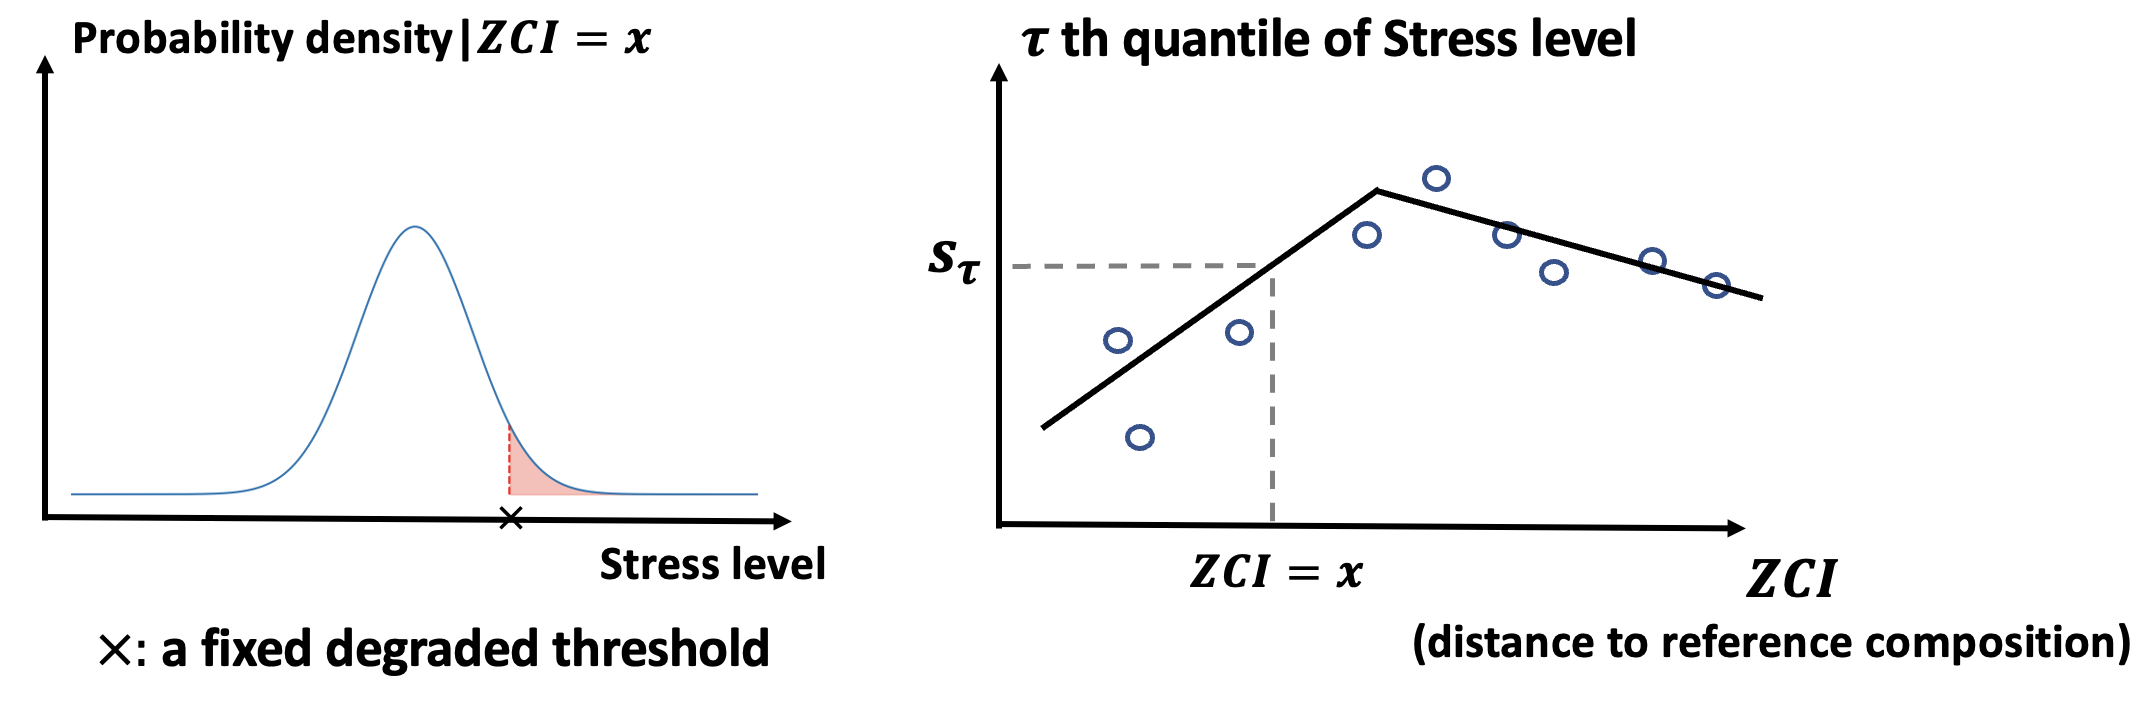
\includegraphics[width=0.9\textwidth]{../presentation/figures/p16_degraded_threshold_and_quantile_regression.png}
\caption{\textit{A pre-fixed degradation threshold on the conditional stress level distribution and the correspondingly predicted quantile value \(\hat s_{\tau}\)}}
\label{fig:p16_degraded_threshold_and_quantile_regression}
\end{figure}


\subsection{Indicator power and robustness with respect to sample size (tentative)}
Power and robustness evaluation of the indicator can be divided into the following specific aims: 
(i) quantify precision of slopes and breakpoint effects and conditional quantiles as sample size varies 
and (ii) estimate power for detecting contamination structure and degradation thresholds, all \emph{within each group $k$}.

	\textbf{Targets:} slopes $\beta_{1,\tau}^{(k)}$, changes $\gamma_{m,\tau}^{(k)}$, breakpoint reliability, pseudo-$R^2$, degradation test (Type I / power), and conditional quantiles $\widehat Q_{\delta X|Z,S}$.

	\textbf{Procedure (tentatively designed steps):}
\begin{enumerate}
    \item \emph{Baseline fit:} Fit full piecewise quantile model (fixed $\kappa_m$, fixed $S_{\text{sel}}$) for $\tau \in \mathcal{T}$; store parameters and residuals; test residual Moran's $I$.
    \item \emph{Bootstrap (uncertainty):} If no residual spatial autocorrelation: site bootstrap; else block bootstrap. Refit using original $S_{\text{sel}}$; derive percentile CIs and relative widths.
    \item \emph{Subsampling (precision curves):} For a grid of reduced sizes $n_k^{(g)}$, draw $R$ subsamples preserving 
    ratio of \(\frac{reference}{disturbed}\); refit; summarize bias and RMSE of slopes / predicted quantiles; locate diminishing returns size.
    % \item \emph{Effective sample size:} When mild spatial correlation persists, report $ n_{k,\text{eff}} = \dfrac{n_k}{1 + (n_k-1)\bar{\rho}_k }$ and inflate SEs by $\sqrt{n_k/n_{k,\text{eff}}}$.
    \item \emph{Power simulation:} \(H_0\): $\beta_{1,\tau}=\gamma_{m,\tau}=0$; \(H_1\): baseline (and reduced effect). Simulate $L$ datasets holding $(z, S_{\text{sel}})$ fixed; estimate power for joint slope/breakpoint test and degradation classification at threshold $x_k^*$.
    \item \emph{Breakpoint reliability:} Accept $\kappa_m$ if CI width $< 0.3$ of ZCI span \emph{and} $\Pr(\gamma_{m,\tau}\neq 0 \text{ for some } \tau) \ge 0.8$; otherwise reduce segments or increase sample size.
    \item \emph{Outputs:} (a) precision and power curves vs. $n_k$; (b) recommended minimum $n_k$ meeting power $\ge 0.8$ (median quantile) and reliability rule; (c) table of median (IQR) parameter estimates.
\end{enumerate}

	\textbf{Interpretation:} Early plateau in precision implies reallocating effort to under-sampled groups or spatial gaps.
     If slopes are consistent but breakpoints unreliable, report continuous gradients instead of thresholds.
    Reliable, sharp breakpoints support categorical management triggers.

